% !TEX root = ./Thesis.tex

\chapter{Background}

\section{Microfluidics}

\subsection{History to present day}

The first analytical miniaturised device fabricated on silicon was presented in 1979 by Terry \textit{et al}
\citep{terry1979ieee}. This device, was a gas chromatograph capable of seperating a simple mixture of gases
in seconds and included an injection valve and a 1.5 m long seperation column. A thermal conductivity detector
was fabricated seperately, and clamped to the silicon wafer containing the column. This subsequently allowed for
a reduction in size of nearly 3 orders of magnitude compared to the conventional lab equipment at the time,
and is regarded \citep{reyes2002micro} as the first demonstration of the power of miniaturisation from which, the
field of lab-on-a-chip and microfluidics would be born.
Into the 1980s, research related to miniaturisation focused on the fabrication of
components, like micropumps \citep{van1988piezoelectric,van1989thermo}, and microvalves \citep{shoji1988prototype},
rather than silicon based analysers.

In 1990, work describing a miniaturised liquid chromatograph on a silicon
wafer was published \citep{manz1990design}. This work described a 5 x 5 mm chip containing a
column and detector that was connected to an off-chip HPLC pump and valves to perform high pressure
liquid chromatography. Concurrently, the concept of a 'miniaturised total analysis system' (µTAS) was introduced
by Manz \textit{et al} \citep{manz1990miniaturized}, where the incorporation of sample pretreatment, separation,
and detection onto a single device was proposed to enhance the analytical performance of the device rather
than to just simply reduce its size. However, it was also recognised that miniaturisation of the device
presented the advantages of not only a smaller consumption of materials, but would also
enable integration of multiple separation techniques capable of monitoring many components in a single device.

Such a device was envisioned as capable of sample handling, analysis, detection, and incorporating control of
mass transport and measurements. Conventional pumps at the time struggled with the high pressures needed for transport
in small channels and early theoretical considerations showed that electroosmotic pumping was an attractive and
feasible way to move aqueous liquid through a µTAS especially when separation was needed.

Electroosmosis is defined as the motion of liquid induced by an applied potential. An electroosmotic pump
has no moving parts and produces an even flow in the entire length of the channel, ideal for early applications
of µTAS that imagined separating and analysing aqueous solutions. Early efforts were first put into optimising
injection and separationg by switching voltages between the reservoirs containing reagent, carrier and
waste \citep{manz1991integrated}.

Electrophoresis in a µTAS was reported in 1992 using silicon and glass \citep{harrison1992capillary}. This
demostrated success in using electroosmotic pumping for flow control in interconnected channels without the
use of valves. The concept of integrating injection, separation, and detection was demostrated. As electrophoresis
is most commonly used to separate biological samples, usually charged molecules in aqueous solution, it started to be
coupled with laser induced fluorescence to detect amino acids separated on-chip \citep{seiler1993planar}. In
addition to separation of biological samples, applications of reactions concerning biomolecules and the
handlng of cells started to emerge.

Microfabricated devices found uses in DNA amplification by polymerase chain reaction
(PCR) \citep{woolley1996functional} and cellular metabolism \citep{bousse1994micromachined}.
As analysis of biological samples in water became available, fabrication of the devices
from glass and silicon became unecessary and inappropriate. Silicon was at the time expensive, but more
importantly, opaque to visible and UV-light and so couldn't be used with conventional methods of optical
detection frequently used in biology. The increasing complexity of the systems meant it became
important for pumps and valves to be integrated into the device these are more easily made from elastomers
than rigid materials. The trend towards studying mammalian cells lead to different requirements such as gas
permeability which neither glass or silicon can provide. This required replacement of silicon and glass with
polymers \citep{RN5}.

Poly(dimethylsiloxane) (PDMS) was the polymer of choice, the properties of which differ greatly
from silicon or glass \citep{ng2002components,whitesides2001flexible}. The switch to PDMS was made even
more attractive by the development of soft-lithography as a method for building prototype
devices \citep{mcdonald2000fabrication} and the development of a method to fabricate pneumatically actuated valves,
pumps, and mixers \citep{mcdonald2000fabrication}. Thse are only possible due to the elastomeric nature of PDMS
and would not be possible with a pure silicon or glass devices.
The improved methods of fabrication lead to the developments of the components required for more sophisticated
experiments in the form of: valves that enabled immunoassays(\fig{fig:immunoassay})\citep{weibel2005torque}; an integrated
microfluidic system for efficient mixing \citep{gunther2005micromixing}; and pumps\citep{laser2004review}.
With these compnents, microfluidics was in a position to tackle more complex problems one example of the complexity is shown in \fig{fig:immunoassay}.


\begin{figure}
  \begin{center}
  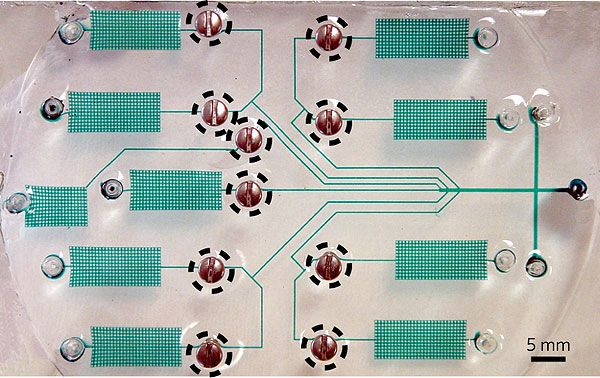
\includegraphics[width=\columnwidth,height=5cm,keepaspectratio]{Torque-immunoassay.jpg}
  \end{center}
  \caption{Coponents of a microfluidic device got increasingly complicated. This device from Ref.\citep{weibel2005torque} performs
  immunoassays - widely used in medical and biological research. The screws (dashed circles) are manually operated valves. Water with green dye
  shows the channels.}
  \label{fig:immunoassay}
\end{figure}


As these fabrication methods become more widely used the field of microfluidics moved, from
adding components to its analytical arsenal, to starting to find applications for devices.
Microfluidic devices then found applications in protein cyrstallisation \citep{hansen2002robust},
separations coupled with mass spectroscopy \citep{ramsey1997generating}, single cell manipulation \citep{wheeler2003microfluidic},
and synthesis of $^{19}$F-labelled organic compounds for use in PET scans \citep{lee2005multistep}.

A subsection of microfluidics began to emerge around this time too, as
low reynolds numbers make multiphase flow manipulation
relatively easy, the generation and manipulation of droplets\citep{thorsen2001dynamic, link2004geometrically, tan2004design} began to be explored.
These involved dispersing a liquid phase in a continuous
liquid stream to form a monodisperse emulsion of (often) aqueous droplets in oil. These droplets
were used to produce polymer particles\citep{nie2005polymer}, in making irregular particles\citep{nisisako2007formation},
hollow microcapsules\citep{utada2005monodisperse}, and protein detection in cells\citep{huebner2007quantitative}. An example of one of the ways droplets were first
produced in microfluidic devices is shown in \fig{fig:IntroDrops}.

\begin{figure}
  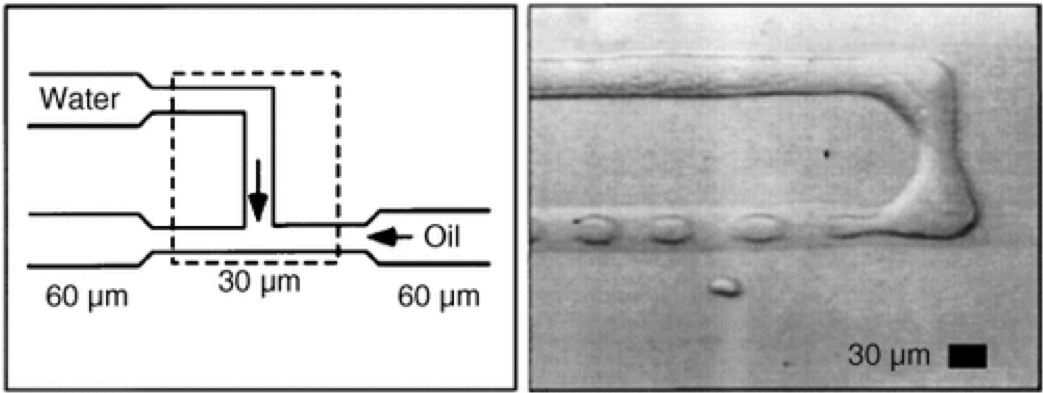
\includegraphics[width=\columnwidth]{Droplets.png}
  \caption{Formation of droplets in a T-Junction of a microfluidic device the continuous hydrocarbon
  phase disperses a water phase. Figure from \citep{RN104}}
  \label{fig:IntroDrops}
\end{figure}

In parallel, another branch of microfluidics was being developed. Its goal was to
culture cells in a repeatable way. In their normal environment, cells are subject to multiple
cues including cytokines and other signalling molecules from neighbouring cells, biochemical
interactions with the extracellular matrix, mechanical stress and direct cell to cell contacts.
Microfluidics was seen as an ideal method of providing cells with these cues in a controlled and reproducible fashion that couldn't be easily
replecated with conventional cell culture, by using microfludic devices one can combine
cell culture with analytical techniques in order to probe the biochemical processes that
govern cell behaviour.

\begin{figure}
  \begin{center}
  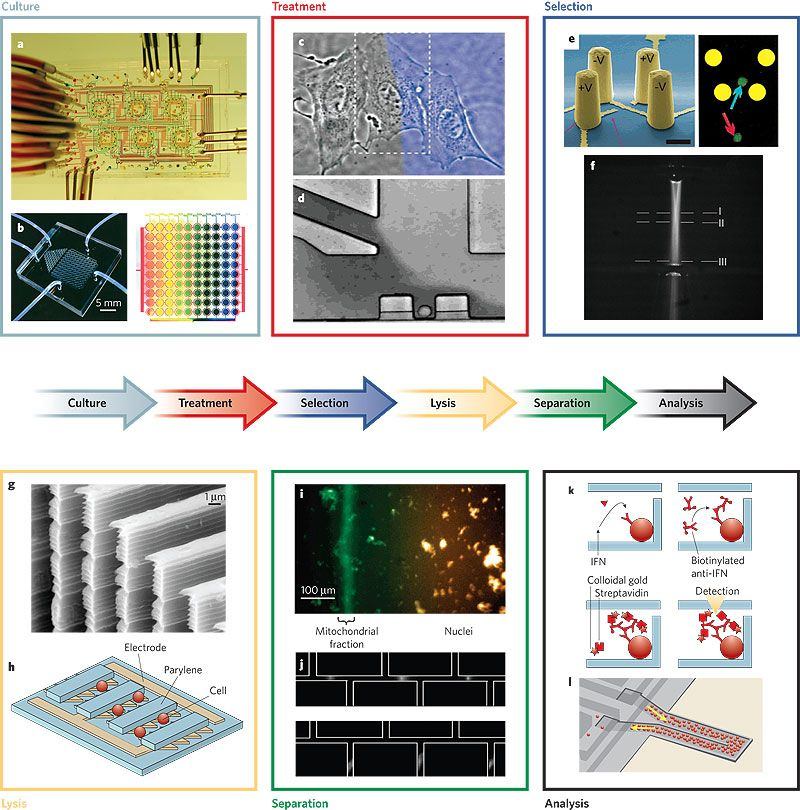
\includegraphics[width=\columnwidth,height=12cm,keepaspectratio]{Microfluidic-Cell-Culture.jpg}
  \end{center}
  \caption{A collection of microfluidic devices that enabled cell based assays from cell culture, to selection and treatment,
  to analysis. \textbf{a}, Six biorexctors are operated in parallel in a single chip to monitor small numbers of cells \citep{balagadde2005long},
  \textbf{b}, Microfluidic cell-culture array with integrated concentration gradient generator (left). Image of concentration
  gradient when blue and yellow dye is used (right) \citep{RN41}. \textbf{c} Two laminar streams exposing two sides of a single cell to different
  conditions \citep{takayama2001laminar}.
  \textbf{d}, Perfusion over a single trapped cell. The perfusion media can be switched in 100 ms \citep{wheeler2003microfluidic}. \textbf{e}, (left) Cell dielectrophoresis
  trap. (right) Fluorescent image of trapped cell indicated by blue arrow \citep{Voldman:2002gf}. \textbf{f}, Fluorescent image of light path at the detection
  zone in a micro flow cytometer \citep{wang2004measurements}. \textbf{g} Scanning electron micrograph of a mechanical lysis device with sharp knife-like protrusions \citep{di2003reagentless}.
  \textbf{h}, Schematic of electrical lysis device with microelectrodes \citep{lee1999micro}. \textbf{i}, Isoelectric focusing of cell organelles \citep{lu2004microfabricated}.
  \textbf{j}, Two-dimensional separation of four model proteins. Isoelectric focusing (top) followed by SDS gel electrophoresis \citep{li2004integration}.
  \textbf{k}, Schematic of immunoassay using microbeads as a solid support \citep{sato2002microchip}. \textbf{l}, Schematic of a hollow cantilever-mased mass sensor
  for analyte detection \citep{burg2003suspended}. Taken from Ref.\citep{el2006cells}}
  \label{fig:CellCulture}
\end{figure}

Microfluidic devices have been used enable cell-based assays from cell culture to biochemical analysis. In
\fig{fig:CellCulture} images of different devices are shown that convey how complex the devices being
produced were becoming, despite integration of functionalities proving difficult, these demonstrate the
power of miniaturisation and the ingenuity being developed in the field.
Microfluidics can offer unique control over cell-cell and soluble cues typical of
\textit{in vivo} cell environments by combining microfabrication of 3D extracellular matrix (ECM)
structres and fluid networks that can deliver nutrients and oxygen \citep{folch1999molding}.

Throughout the 2000s, microfabrication, which combined micropatterning techniques such as
photolithography, photoreactive chemistry, and soft lithography, made it possible to engineer the
microenvironment of the cell on similar length scales to the cell itself \citep{folch2000microengineering}. This surface
patterning of micrometre sized features enabled control of cell-EDM interactions and was used
to fabricate 3D scaffolds on which to grow cells that were made of biodegradable
materials \citep{tsang2004three}.

One area of application was the 3D culture of liver cells. \textit{In vitro} culture
of liver cells is of particular interest as many drugs fail clinical studies because they
either damaged the liver directly, or because the metabolites produced by the liver are toxic
\citep{sivaraman2005microscale}. Efforts were made to produce \textit{in vitro} culture
systems that mimic real liver conditions. In the liver, hepatocytes are found in a complex
3D environment in which nutrients, soluble factors and oxygen are transported through blood
capillaries and bile canaliculi. This 3D environment often contains polar tissue structure
where two sides of the cell are exposed to different media, for example, in the liver
some hepatocytes are exposed to the bile on one side and blood on the other. This polar structure
is hard to reproduce using 2D cell culture alone. Using silicon as a substrate, Powers \textit{et al} fabricated
3D liver reactors using array of 300 µm wide channels \citep{powers2002microfabricated}. In their
device they perfused rat liver cells providing fluid shear stresses at physiological range. They found
that the cells seeded into the channels rearranged extensively to form 'tissue like' structures and
remained viable for up to 2 weeks.

Later, Sivaraman \textit{et al} developed a different system to culture liver cells in a 3D scaffold,
using a polycarbonate housing for a silicon device that contained microfabricated wells in which the
cells were seeded and perfused with media. They also found that the cells in the 3D culture
also had cell-cell contacts that resembled those found in tissues \textit{in
vivo} \citep{sivaraman2005microscale}. It has been observed that co-culture of hepatocytes with other cell types,
inculding liver epithelial cells and Kupffer cells, prolongs the survival of cultured hepatocytes and helps maintain
liver-specific properties such as albumin secretion \citep{guguen1983maintenance}.

As 3D cell culture became more widely used, a new subgenre of microfluidics was formed, organ-on-a-chip. Early efforts had shown
that microfabrication of adhesive substrates provided well-controlled environments for cell growth and epression of differentiated tissue-specific functions
\citep{chen1997geometric,bhatia1999effect}. Advances in soft lithography-based microfluidic devices made it easier
to develop the more complex 3D architecture of living tissues and organs. For example, a poly(dimethylsiloxane) (PDMS) device
that contained structures that mimic the structure of the endothelial-epithelial interface that forms the liver sinusoid \citep{nakao2011bile}.

Along with liver function, kidney, lung, and body functions were replicated in microfluidic devices shown in \fig{fig:OrganChip}. Whilst the liver and kidney offer highly
simplified microengineered models, within organs \textit{in vivo} nutrients, hormones, metabolites, cytokines and physical signals are usually transferred across interfaces
between adjacent living cells and therefore require a much more complex microenvironment
for true replication. Huh \textit{et al} created a model of the human alveolar-capillary interface formed in a flexible
PDMS device containing a central channel and two hollow side chambers \citep{huh2010reconstituting}. A 10 µm thick PDMS membrane containing an
ordered array of micropores (10 µm diameter) was stretched across the central channel, splitting it in two see \fig{fig:OrganChip}.
Human alveolar epithelial cells were then cultured on
one side of the membrane and exposed to air, while human lung capillary endothelial cells were cultured on the opposing side and exposed to flowing
medium. When the holllow side chambers were exposed to vacuum, the cells were subjected to strain ranging from 5\%-15\% to match strain observed within
whole lung \textit{in vivo}. In doing so, they found their 'lung on a chip' accentuated the inflammatory responses of the cells to silica
nanoparticles. This mechanical strain also enhanced uptake of nanoparticles and stimulated the transport into the vascular channel and
similar effects of physiological breathing were observed in whole mouse lung. These early organ on chip experiments paved the way for more complex
'Body-on-a-chip' devices that contain multiple types of cultured cells connected by a network of
microfluidic channels that permit recirculation and exchange of metabolites in a physiologically-relevant manner \citep{esch2011role} and
has found applications in drug screening and disease modelling \citep{skardal2016organoid}.


\begin{figure}
  \begin{center}
  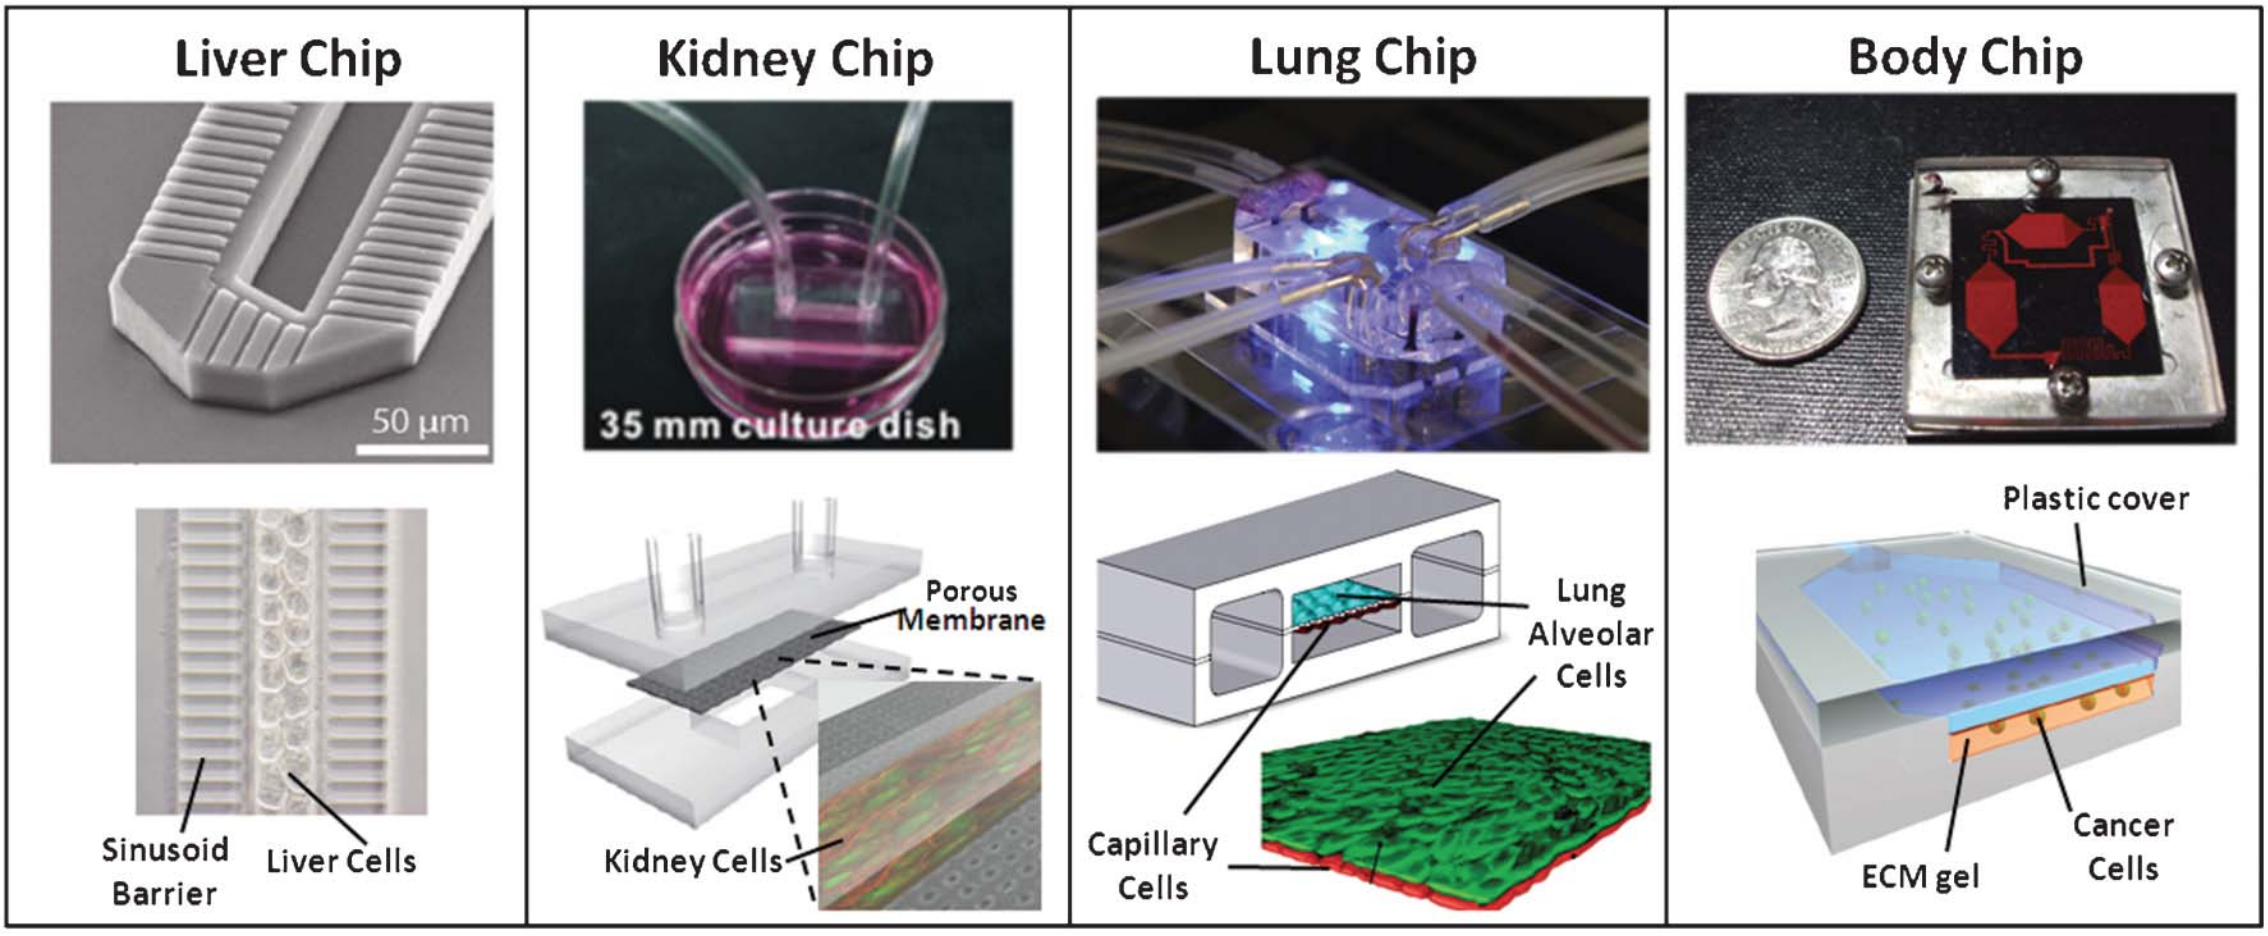
\includegraphics[width=\textwidth]{Organ-on-a-chip}
  \end{center}
  \caption{Organ-Organ and tissue-tissue interfaces in microdevices. Liver chip: A microfluidic liver device with cell culture and flow chambers separated by
  a baffle that separates cultured hepatocytes from fluid flow to simulate the endothelial-hepatocyte interface of the liver sinusoid. This geometry promotes alignment
  of hepatocytes in two lines that facilitates the production of functional bile canaliculi along hepatic-cord-like structures\citep{nakao2011bile}. Kidney chip:
  A simple kidney on a chip that mimics the interface between epithelium and flowing urine was created by donding a PDMS well and a PDMS channel to either side
  of a semi-permeable membrane on which cells are cultured and subejected to fluid flow\citep{jang2010multi}. Lung chip: A lung-on-a-chip capable of replicating mechanical
  strain caused by breathing, fabricated from PDMS that mimics the physiological function of the alveolar-capillary interface in the human lung. The hollow chambers
  are subjected to cyclic suction to replicate breathing movements whilst fluid flowing mimics blood flow\citep{huh2010reconstituting}. Body chip: A
  microfluidic device containing multiple linked tissue types representing different organs was conctructed by sealing three cell culture chambers against a cover. Each
  cell culture chamber contains a 3D ECM gel containing living cells from a different organ. Media was circulated through the chambers via microfluidic channels
  during operation\citep{sung2009micro}. Figure taken from \citep{huh2012microengineered}.}
  \label{fig:OrganChip}
\end{figure}

As the complexity of cell culture within microfludic devices increased, so to, did the detection methods. Coupling
a dector to an LOC is critical for any analytical purpose. A number of detector technologies were demonstrated in
microfluidic devices including electrochemical\citep{wang2006electrochemical}, mechanical \citep{raiteri2001micromechanical},
and optical methods \citep{kuswandi2007optical}. The small sample volumes typical to a microlfuidic experiment
are an important challenge to overcome for any detector, ideally, a detector should be highly sensitive and scalable
to smaller dimensions.

The mechanism and features of the detection technologies summarised in \citep{pires2014recent} and
reproduced in Table \ref{tab:detectors}.

\newpage

\begin{table}
\begin{center}
    \label{tab:detectors}
    \begin{tabular}{|p{5cm}||p{5cm}||p{5cm}|}\hline\hline
      Method & Mechanism & Features \\ \hline
      Electrochemical & Measures changes in conductance, resistance and/or capacitance at the active surface of the elctrodes  &
      (+) Real-time detection, (+) Low-cost microelectrode fabrication, (-) Control of ionic concentrations before detection, (-) Short sehelf life  \\ \hline
      Mechanical & Detection is based on variations of the resonant frequency or surface stress of the mechanical sensor &
      (+) Monolithic sensor integration, (+) Label free detection, (-) damping effects in liquid samples, (-) Detection takes time (~30 mins), (-) Complex fabrication  \\ \hline
      Optical & Detects variations in light intensity, refractive index sensitivity, or interference pattern &
      (+) Minimal sample preparation, (+) Real-time detection, (+) Ubiquitous in laboratories, (-) Conventional instrumentation is expensive, (-) Set-up complexity \\ \hline\hline
    \end{tabular}
\caption{Summary of electrochemical, mechanical and optimal deteciton technologies employed in microfluidics.}
\end{center}
\end{table}

Electrochemical detection involves the interaction of chemical species with electrodes or probes. This interaction
results in a variation of signal, such as potential or current, which enables analysis of target analytes. The
electrochemical phenomenon deals with two major effects: (i) chemical reactions are promoted by passing an
electrical current through the electrode system; or (ii) electrode responses are triggered due to specific chemical reactions. These
effects are usually observed using an eletrolytic cell. Reactions of oxidation and reduction occurring at the surface of the electrodes
are the basis for electron transfers between the electrolyte (sample) and the electrodes. In a typical
electrolytic cell, the electrode system is formed by the working electrode where detection of a certain
analyte is analyzed, and the reference electrode where a standard oxidation/reduction is conducted \citep{flanagan2005electrochemical}.
Wongkaew \textit{et al} reported an electrochemical biosensor that employed microelectrode array. In
the array, adjacent electrode fingers form micro-sized gaps which allow an increase of the diffusion flux
of chemical species, thus leading to an enhanced collection efficiency and higher signal amplification.
The microchannels of the device were made by hot embossing PMMA and the electrodes were made by e-beam
and wet-etching processes. The detection of targets using this system took 250 seconds and reported
limit of detection of 12.5 µM.

Mechanical detection systems mainly used cantilever technology, which showed that it could be accurate
when detecting biomolecules \citep{waggoner2007micro}. Cantilever-based devices generally operate in two
different modes upon analyte binding: (i) static deflection, where binding on one side of a cantilever
causes unbalanced surface stress resulting in a measurable deflection; (ii) dynamic, resonant mode, where
binding on a cantilever causes variations of its mass and consequently shifts the resonant frequency.
Mechanical-based detection may require no labelling of biomolecules. Labels often make the detection
method more complicated, time-consuming and costly, and could interfere with the function of biomolecules
under investigation. Anoter characteristic of cantilever technology is the potential to fabricate large
arrays of sensors for multi-molecular sensing \citep{ferrari2005cancer}. Hou \textit{et al} \citep{hou2013aptamer} presented
a device that contained a microfabricated canter lever array  for the  specific detection of
oxytetracycline (OTC), a common broadband antibiotic used in animals that can accumulate in our food chain
and cause side effects on humans. The device achieved this by functionalising the cantilvers with OTC
specific DNA aptamers which bind to the OTC and icrease the load on the cantilevers and causes them
to deflect and once calibrated can indicate the concentration of OTC in solution. The limit of detection
in this case is 0.2 nM in 1000 seconds.

Optical detection is preferred for robust, sensitive Lab on a chip devices it has been the most widely
used technique for quantitative proteomic analysis \citep{rusling2010measurement} and infectious disease
diagnostics \citep{foudeh2012microfluidic}, due, in part, to the ubiquity of the optical instrumentation
required in biological laboratories meaning these devices can be used readily in most locations.
Conventional optical detection methods, including absorbance \citep{wang2011integration},
chemiluminescence \citep{wojciechowski2009organic}, fluorescence \citep{yildirim2012aptamer}, and surface
plasmon resonance (SPR) \citep{foudeh2014sub}, have all been applied in microfluidic devices. Foudeh
\textit{ et al} \citep{foudeh2014sub} developed an SPR microdevice for the detection of
\textit{Legionella pneumophila} which is the pathogenic organism that causes Legionellosis, and
is responsible for fatality rates over 10\% within hospital and indutrial outbreaks
\citep{swanson2000legionella}. The device is ultra-sensitive to RNA of \textit{Legionella pneumophila}
and has a limit of detection of 1 pM in less than 3 hours.

Presently, Microfluidics is a large and diverse field, so much so that the areas that started out as sub-categories are now referred to as their
own field of research, indeed, within the last three years the journal Lab on a Chip has published no less than 116 reviews focusing on a wide variety of applications
that microfluidics now enjoys such as: 3D printed fluidic networks\citep{kinstlinger20163d}; droplet microfluidics for synthetic biology\citep{gach2017droplet};
phase behaviour characterization for industrial CO$_2$, oil and gas\citep{bao2017microfluidic}; the production of stem cells using messenger RNAs\citep{giulitti2019direct};
and paper microfluidics for diagnosis of malraia in low resource community\citep{reboud2019based}.

\newpage

\section{NMR theory}\label{Quantum}

\subsubsection{Nuclear Spin}\label{Spin}

Nuclei have an intrinsic property known as spin. This spin can be represented by operators
along the three Cartesian axes $\hat{I}_x$, $\hat{I}_y$, and $\hat{I}_z$ where:
\begin{align}
  \hat{I}_x\quad=&\quad-i\hbar(y\frac{\partial}{\partial{z}}-z\frac{\partial}{\partial{y}})\\
  \hat{I}_y\quad=&\quad-i\hbar(z\frac{\partial}{\partial{x}}-x\frac{\partial}{\partial{z}})\\
  \hat{I}_z\quad=&\quad-i\hbar(x\frac{\partial}{\partial{y}}-y\frac{\partial}{\partial{x}})
\end{align}

The commutation relation between two operators is defined as:
\begin{equation}
  [\hat{A},\hat{B}] = \hat{A}\hat{B} - \hat{B}\hat{A}
\end{equation}

If $[\hat{A},\hat{B}] = 0$ the operators are said to commute. The physical implication
of this is that the two observables can be measured at the same time. Measuring one
does not affect the outcome of the other and vice versa.

The spin operators $\hat{I}_x$, $\hat{I}_y$ and $\hat{I}_z$
have cyclic commutation rules:
\begin{align}\label{eqn:commutator}
  [\hat{I}_x,\hat{I}_y] = i\hat{I}_z\\
  [\hat{I}_y,\hat{I}_z] = i\hat{I}_x\\
  [\hat{I}_x,\hat{I}_z] = i\hat{I}_y
\end{align}

This cyclic commutation means that the spin that nuclei posses can be treated as a
type of angular momentum and in NMR, $\hat{I}_x$, $\hat{I}_y$ and $\hat{I}_z$ are
referred to as the spin angular momentum operators.

The total square angular momentum operator, $\hat{I}^2$ can be defined as:
\begin{equation}
  \hat{I}^2 = \hat{I}_x^2 + \hat{I}_y^2 + \hat{I}_z^2
\end{equation}

This commutes with the three spin angular momentum operators:
\begin{align}\label{eqn:I2commute}
  [\hat{I}^2,\hat{I}_x] = 0\\
  [\hat{I}^2,\hat{I}_y] = 0\\
  [\hat{I}^2,\hat{I}_z] = 0
\end{align}

Operators act on states. To explain this, consider a generic operator $\hat{B}$ with eigenstates $\ket{x}$ and $\ket{y}$. When a state is acted upon by an operator it is denoted by:
\begin{equation}
  \hat{B}\ket{x} = b\ket{x}
\end{equation}

the same state is returned, multiplied by some scalar $b$, that is an eigenvalue of $\ket{x}$
in the operator basis B.

Analagous to this, spin angular momentum operators have eienstates and eigenvalues. If the nuclear spin quantum number is $I$, then the operator $\hat{I}_z$ has $2I+1$
eiegenstates, $m_I$. State are denoted $\ket{I,m_I}$\citep{dirac_1939} and the angular momentum operator acts according to the following:
\begin{equation}
  \hat{I}_z\ket{I,m_I} = m_I\hbar\ket{I,m_I}
\end{equation}

The total square angular momentum acts in the following way:
\begin{equation}
  \hat{I}^2\ket{I,m_I} = I(I+1)\hbar\ket{I,m_I}
\end{equation}
for a nuclear spin state, $I$ can take half-integer and integer values for zero i.e
$I = 0,\frac{1}{2},1,\frac{3}{2}\dots$, $m_I$ takes one of the integer values from $-I
\text{to} +I$.

\subsubsection{Spin Systems}\label{SpinStates}

The simplest case that can be considered in NMR is a system of isolated
spin-1/2 nuclei.

According to the quantum theory of angular momentum discussed in \ref{Spin}, a
single spin-1/2, when placed in a magnetic field has two eigenstates of angular
momentum along the $z$-axis, denoted by $\ket{\alpha}$ and $\ket{\beta}$ and defined
as:
\begin{align}
  \ket{\frac{1}{2},+\frac{1}{2}} = \ket{\alpha}\\
  \ket{\frac{1}{2},-\frac{1}{2}} = \ket{\beta}
 \end{align}

The states $\ket{\alpha}$ and $\ket{\beta}$ are called the \textit{Zeeman eigenstates}
of a spin-1/2 and are acted on by $\hat{I}_z$ according to the following:
\begin{align}\label{eqn:momentum}
  \hat{I}_z\ket{\alpha} = +\frac{1}{2}\hbar\ket{\alpha}\\
  \hat{I}_z\ket{\alpha} = -\frac{1}{2}\hbar\ket{\beta}
\end{align}

\eqn{eqn:momentum} shows that the eigenstate $\ket{\alpha}$ has an eigenvalue of
$+\hbar/2$ and $\ket{beta}$ has an eigenvalue of $-\hbar/2$ these are said to
be polarized along the $z$-axis. This polarisation is represented in
\fig{fig:Projection} by the up and down arrows pointing along the positive
or negative $z$-axis indicating the direction of well-defined spin angular momentum.
These arrows should not be overinterpreted as for the same spin,
the $x$ and $y$ companents are fundamentally unpredicatble
since the states $\ket{\alpha}$ and $\ket{\beta}$ are not eigenstates of the operators
$\hat{I}_x$ or $\hat{I}_y$. The arrow along the $z$-axis does not mean the
$x$-axis angular momentum is zero. The $x$-axis angular momentum is \textit{undefined}
as measurments give $±1/2$ with equal probability and this is very hard to represent
in a diagram.

\begin{figure}
  \begin{center}
  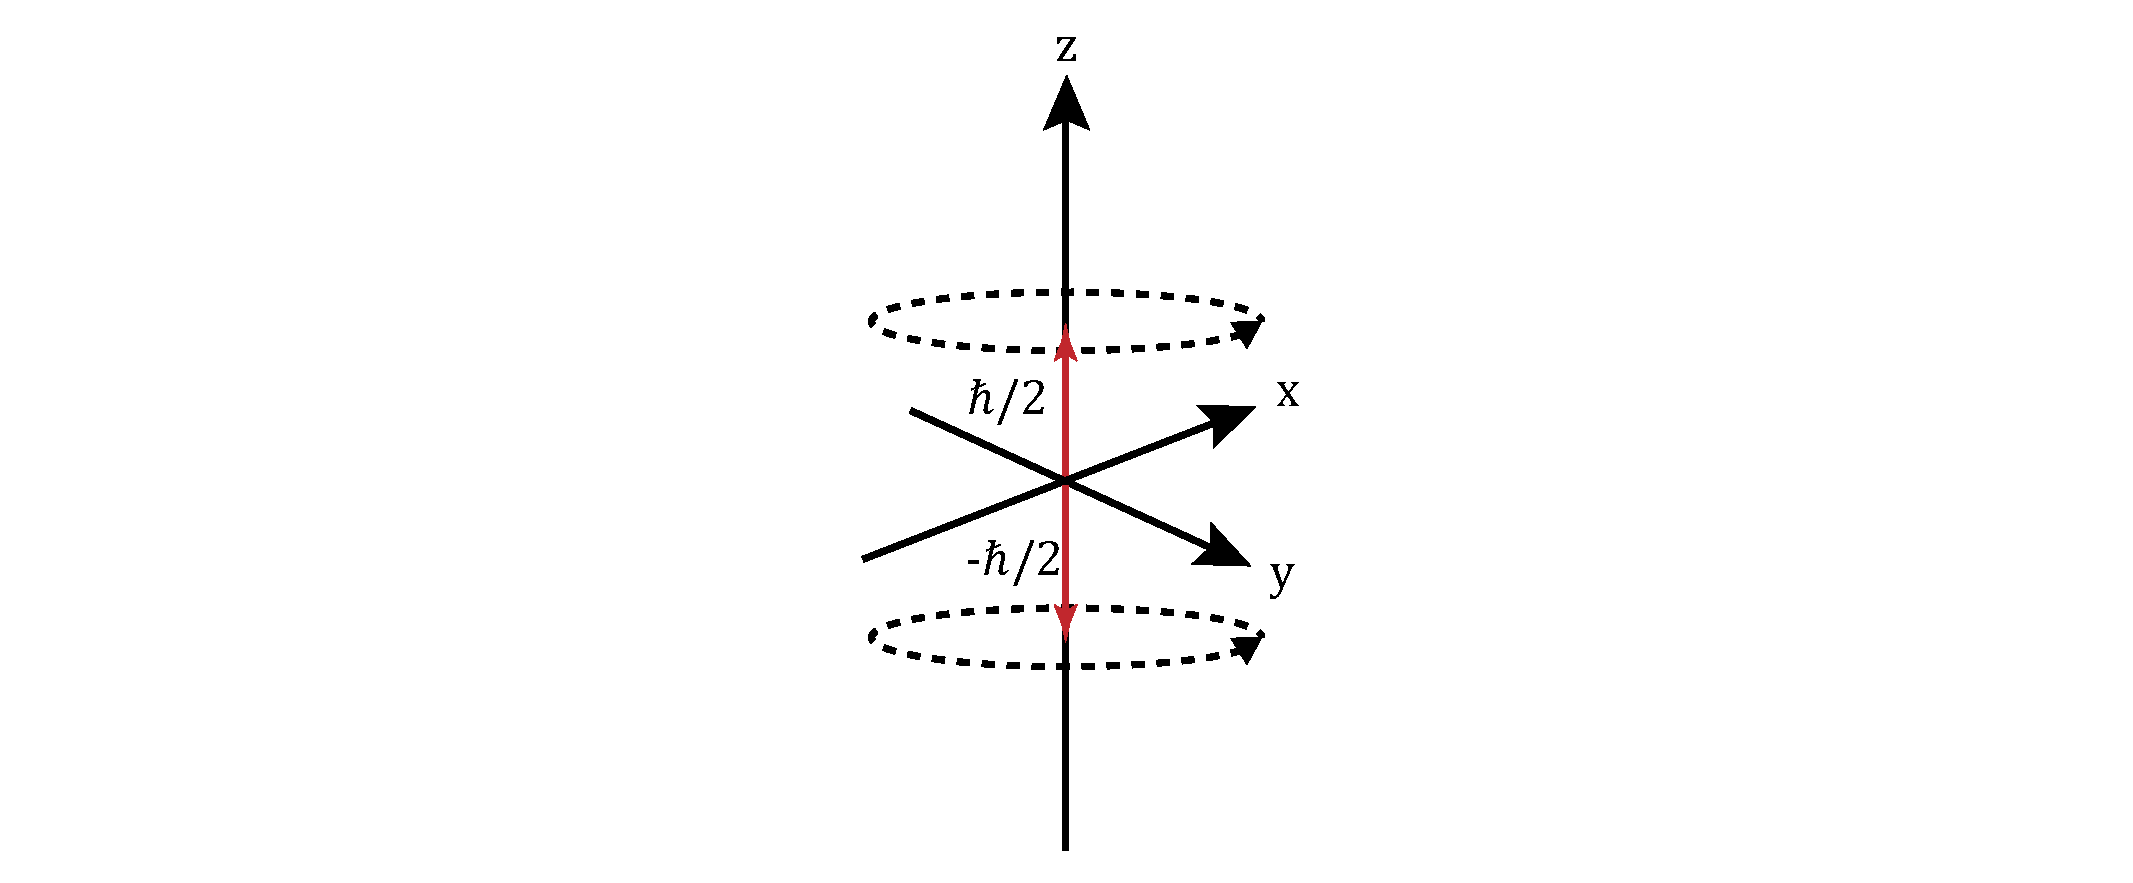
\includegraphics[width=\columnwidth,height=5cm,keepaspectratio]{StateProjection.pdf}
  \end{center}
  \caption{The projection of the two zeeman eigenstates in a spin 1/2 nucleus.}
  \label{fig:Projection}
\end{figure}


The zeeman eigenstates can be used to define the Zeeman basis. The two kets, $\ket{\alpha}$ and $\ket{\beta}$ can be represented by the column vectors:

\begin{equation}
  \ket{\alpha} = \begin{pmatrix}
    1\\
    0
\end{pmatrix}\quad
 \ket{\beta} = \begin{pmatrix}
   0\\
   1
\end{pmatrix}
\end{equation}

as well as kets, bras are also defined by taking the conjugate transpose of the ket, $\ket{\alpha}^{\dagger} =
\bra{\alpha}$ such that
\begin{equation}
  \bra{\alpha} = \begin{pmatrix}
    1 & 0
\end{pmatrix}
  \bra{\beta} = \begin{pmatrix}
  1 & 0
\end{pmatrix}
\end{equation}

The state, $\ket{\psi}$, of a two level system can now be completely decribed in this basis
as the linear combination of the basis states:
\begin{equation}\label{eqn:zeeman}
  \ket{\psi} = c_1\ket{\alpha} + c_2\ket{\beta} = \begin{pmatrix}
    c_1\\
    c_2
\end{pmatrix}
\end{equation}
\begin{equation}
  \bra{\psi} = c_1^*\bra{\alpha} + c_2^*\bra{\beta} = \begin{pmatrix}
    c_1^* & c_2^*
\end{pmatrix}
\end{equation}

These are normalised such that $c_1c_1^* + c_2c_2^* = 1$.

To complete the picture, the states must be orthonormal. Orthonormality between states exists if the inner product of the basis states $\ket{r_i} ~\text{and}~ \ket{r_j}$ satisifies the following conditions:

\begin{equation}
  \langle r_i\vert r_j\rangle = \delta_{ij}
\end{equation}

where the Kronecker delta, $\delta_{ij}$ is:
\begin{equation}
  \delta_{ij} = \begin{cases}
    0 & ~\text{if}~ i \ne j\\
    1 & ~\text{if}~ i = j
                \end{cases}
\end{equation}

where $\langle r_i\vert r_j\rangle = \delta_{ij}$ denotes taking the dot product between the two
vectors $\ket{r_i}$ and $\ket{r_j}$.

The basis states help to quantify the component of a state vector along that state. Take our example from \eqn{eqn:zeeman}, we can construct inner products of the overall state, $\ket{\psi}$ with $\ket{\alpha}$ and $\ket{\beta}$ to determine component of the basis states.
\begin{equation}
  \langle\alpha\vert\psi\rangle = c_1 \quad \langle\beta\vert\psi\rangle = c_2
\end{equation}

The outer product of the basis state, $\ket{r_n}$, for an N-spin system must satisfy:
\begin{equation}
  \sum_{n=1}^{N} \ket{r_n}\bra{r_n} = \mathbb{1}
\end{equation}

where $\mathbb{1}$ is an N by N identity matrix.

When a second spin is introduced, the Hilbert space is extended to accommodate additional spin
states by taking the tensor product of the basis states


\begin{align}\label{eqn:2spinstates}
\ket{\alpha_{1}\alpha_{2}} = \ket{\alpha_1} \otimes \ket{\alpha_2} = \begin{pmatrix}
  1\\
  0\\
  0\\
  0
\end{pmatrix} &\quad
\ket{\alpha_{1}\beta_{2}} = \ket{\alpha_1} \otimes \ket{\beta_2} = \begin{pmatrix}
  0\\
  1\\
  0\\
  0
\end{pmatrix}\\
\ket{\beta_{1}\alpha_{2}} = \ket{\beta_1} \otimes \ket{\alpha_2} = \begin{pmatrix}
  0\\
  0\\
  1\\
  0
\end{pmatrix} &\quad
\ket{\beta_{1}\beta_{2}} = \ket{\beta_1} \otimes \ket{\beta_2} = \begin{pmatrix}
  0\\
  0\\
  0\\
  1
\end{pmatrix}
\end{align}
The subscripts indicate which spin we are reffering to, e.g. $\ket{\beta_1\alpha_2}$ means that
spin 1 is in the $\beta$ state and spin 2 is in the $\alpha$ state.

\subsubsection{Pauli matrices and more Operators}

In quantum mechanics each observation is associated with a particular operator. For
example, the measurement of the spin angular momentum along the $z$-axis is associated with
$\hat{I}_z$ and when applied to the $\ket{\alpha}$ gives the result seen in \eqn{eqn:momentum}. The
probability of obtaining this result is 1 as $\ket{\alpha}$ is an eigenstate of $\hat{I}_z$. In
all other cases the results follow statistical laws and the result of an individual experiment
is unpredictable.

In quantum mechanics there is a formula for the average result of very many observations, this is
called the expectation value of a general operator, $\hat{A}$, when applied to a spin-1/2 system, $\ket{\psi}$
is denoted:
\begin{equation}
  \langle\hat{A}\rangle = \bra{\psi}\hat{A}\ket{\psi}
\end{equation}

from the genral case listed in \eqn{eqn:zeeman} this becomes:
\begin{align}\label{eqn:expectation}
  \langle\hat{A}\rangle =& \bra{\psi}\hat{A}\ket{\psi}\\
  =& \begin{pmatrix}
    c_1^* & c_2^*
\end{pmatrix}
\begin{pmatrix}
A_{11} & A_{12}\\
A_{21} & A_{22}
\end{pmatrix}
\begin{pmatrix}
  c_1\\
  c_2
\end{pmatrix}\\
=& c_1c_1^*A_{11} + c_1c_2^*A_{12} + c_2c_1^*A_{21} + c_2c_2^*A_{22}
\end{align}

The end sum of all these products is the expectation value of a single spin 1/2 particle when
acted upon by $\hat{Q}$. This quickly becomes cumbersome should there be more than one spin. An easier
way to deal with expectation values is described in \ref{Density}

In NMR we use three operators to determine the projection of angular momentum along a
specific axis, $\hat{I}_x$, $\hat{I}_y$, and $\hat{I}_z$. These are defined by the
Pauli matrices in the Zeeman basis multiplied by $\frac{\hbar}{2}$.

\begin{equation}
  \hat{I}_x=\frac{\hbar}{2}\begin{pmatrix}
    0 & 1\\
    1 & 0
\end{pmatrix}\quad
\hat{I}_y=\frac{\hbar}{2i}\begin{pmatrix}
  0 & 1\\
  -1 & 0
\end{pmatrix}\quad
\hat{I}_z=\frac{\hbar}{2}\begin{pmatrix}
  1 & 0\\
  0 & 1
\end{pmatrix}
\end{equation}

as an example, let's take the example from before of a spin-1/2 particle in a magnetic field
and see what happens if we were to project the $\ket{\alpha}$ state along the z-axis.
\begin{equation}\label{eqn:operators}
  \hat{I}_z\ket{\alpha} = \frac{\hbar}{2}\begin{pmatrix}
    0 & 1\\
    1 & 0
\end{pmatrix}
\begin{pmatrix}
  1\\
  0
\end{pmatrix} = \frac{\hbar}{2}\begin{pmatrix}
  1\\
  0
\end{pmatrix} = \frac{\hbar}{2}\ket{\alpha}
\end{equation}
We find that $\frac{\hbar}{2}$ is the eigenvalue of $\ket{\alpha}$ for the operator $\hat{I}_z$.

We will now examine three more operators and explore how they act on states. They are the total square angular momentum, $\hat{I}^2$ and the two shift operators $\hat{I}^+$ and $\hat{I}^-$ defined as the following:

\begin{align}
  \hat{I}^2 =& \hat{I}_x^2 + \hat{I}_y^2 + \hat{I}_z^2\\
  \hat{I}^+ =& \hat{I}_x + i\hat{I}_y\\
  \hat{I}^- =& \hat{I}_x - i\hat{I}_y
\end{align}
They act on general states according to:
\begin{align}
  \hat{I}^2\ket{I,m_I} =& I(I+1)\hbar\ket{I, m_I}\\
  \hat{I}^+\ket{I,m_I} =& \sqrt{(I(I+1)-m_I(m_I+1))}\ket{I,m_{I+1}}\\
  \hat{I}^-\ket{I,m_I} =& \sqrt{(I(I+1)-m_I(m_I-1))}\ket{I,m_{I-1}}
\end{align}
Using a spin-1/2 particle in a magnetic field as an example we'll let these operators act on the $\ket{\alpha}$ and $\ket{\beta}$ states
\begin{align}
  \hat{I}^2\ket{\alpha} =& \frac{3}{4}\hbar\ket{\alpha}\\
  \hat{I}^+\ket{\alpha} =& 0\\
  \hat{I}^-\ket{\alpha} =& \ket{\beta}\\
  \hat{I}^+\ket{\beta} =& \ket{\alpha}\\
  \hat{I}^-\ket{\beta} =& 0
\end{align}
As the '+' and '-' denote raising or lowering $m_I$ by 1.

As shown in \eqn{eqn:commutator} the three angular momentum opperators cyclically
commute. This means the \textit{sandwich formula} applies.

In general if $\hat{A}$, $\hat{B}$ and $\hat{C}$ cyclically commute then:
\begin{equation}
  \text{exp}\{-i\theta\hat{A}\}\:\hat{B}\:\text{exp}\{+i\theta\hat{A}\} = \hat{B}\cos{\theta} + \hat{C}\sin{\theta}
\end{equation}

geometrically, this can be thought of as a rotation of $\hat{B}$ by $\hat{A}$ through
an angle $\theta$.

It is important to define a set of rotation operators as these are essential for the generation of signal in NMR. They are defined as the complex exponentials of the
angular momentum operators seen in \ref{Spin}:
\begin{align}\label{eqn:RotOp}
  \hat{R}_x(\theta) = exp\{-i\theta\hat{I}_x\}\\
  \hat{R}_y(\theta) = exp\{-i\theta\hat{I}_y\}\\
  \hat{R}_z(\theta) = exp\{-i\theta\hat{I}_z\}
\end{align}
 and they too have matrix representations:
 \begin{align}\label{eqn:RotMat}
   \hat{R}_x(\theta)& = \begin{pmatrix}
      \cos(\frac{1}{2}\theta) & -i\sin(\frac{1}{2}\theta)\\
      -i\sin(\frac{1}{2}\theta) & \cos(\frac{1}{2}\theta)
 \end{pmatrix}\\
 \hat{R}_y(\theta)& = \begin{pmatrix}
    \cos(\frac{1}{2}\theta) & \sin(\frac{1}{2}\theta)\\
    \sin(\frac{1}{2}\theta) & \cos(\frac{1}{2}\theta)
\end{pmatrix}\\
\hat{R}_x(\theta)& = \begin{pmatrix}
    \text{exp}\{-i\frac{1}{2}\theta\} & 0\\
    0 & \text{exp}\{+i\frac{1}{2}\theta\}
\end{pmatrix}
 \end{align}


The rotation operators are applied to to the angular momentum operators using the sandwich formula:
\begin{equation}
  \hat{R}_x(\theta)\hat{I}_z = \text{exp}\{-i\hat{I}_x\theta\}\hat{I}_z\text{exp}\{+i\hat{I}_x\theta\}
\end{equation}

The result of this is a rotation of $\hat{I}_z$ around the $x$-axis by an angle $\theta$:
\begin{equation}
  \hat{R}_x(\theta)\hat{I}_z = \cos{\theta}\hat{I}_z - \sin{\theta}\hat{I}_y
\end{equation}

The rotational direction (sign of the $\sin{\theta}$ term) is determined by the right hand co-ordinate system defined in \eqn{eqn:commutator}.

How each rotational operator transforms the spin angular momentum operators is shown
below:
\begin{equation}
  \hat{R}_x(\theta) \begin{cases}
    \hat{I}_x \rightarrow \hat{I}_x \\
    \hat{I}_y \rightarrow \hat{I}_y\cos\theta + \hat{I}_z\sin\theta \\
    \hat{I}_z \rightarrow \hat{I}_z\cos\theta - \hat{I}_y\sin\theta
\end{cases}
\end{equation}
\begin{equation}
  \hat{R}_y(\theta) \begin{cases}
    \hat{I}_x \rightarrow \hat{I}_x\cos\theta - \hat{I}_z\sin\theta \\
    \hat{I}_y \rightarrow \hat{I}_y \\
    \hat{I}_z \rightarrow \hat{I}_z\cos\theta + \hat{I}_y\sin\theta
\end{cases}
\end{equation}
\begin{equation}
  \hat{R}_z(\theta) \begin{cases}
    \hat{I}_x \rightarrow \hat{I}_x\cos\theta + \hat{I}_y\sin\theta \\
    \hat{I}_y \rightarrow \hat{I}_y\cos\theta - \hat{I}_x\sin\theta \\
    \hat{I}_z \rightarrow \hat{I}_z
\end{cases}
\end{equation}


\subsubsection{Density Operator}\label{Density}

In \eqn{eqn:expectation} we saw how the expectation value of an operator can be expressed as
the product of the matrix represntations of the state and the operator. We can simplify this by
constructing a matrix of the quadratic products of the superposition coeffecients. If in the
general case
\begin{align}
\ket{\psi} =& \begin{pmatrix}
    c_1\\
    c_2
\end{pmatrix} = c_1\ket{\alpha} + c_2\ket{\beta}\\
\bra{\psi} =& \begin{pmatrix}
  c_1^* & c_2^*
\end{pmatrix} = c_1^*\bra{\alpha} + c_2^*\bra{\beta}
\end{align}

Then the matrix has the form:
\begin{equation}
\ket{\psi}\bra{\psi} = \begin{pmatrix}
    {c_1c_1^*} & {c_1c_2^*}\\
    {c_2c_1^*} & {c_2c_2^*}
\end{pmatrix}
\end{equation}

The expectation value of the operator $\hat{A}$ can now be expressed as:
\begin{equation}
  \langle\hat{A}\rangle = \text{Tr}\{\ket{\psi}\bra{\psi}\hat{A}\}
\end{equation}

If there are now two spins we need to consider with states, $\ket{\psi_1}$ and $\ket{\psi_2}$ the
result of measuring $A$ is still uncertain but we can now write an expression for the most likely outcome, $A_obs$
using the sum of expectation values:
\begin{equation}
  A_{\text{obs}} = \bra{\psi_1}\hat{A}\ket{\psi_1} + bra{\psi_2}\hat{A}\ket{\psi_2}
\end{equation}
which can be rewritten using the simplification:
\begin{equation}
  A_{\text{obs}} = \text{Tr}\{(\ket{\psi_1}\bra{\psi_1}+\ket{\psi_2}\bra{\psi_2})\hat{A}\}
\end{equation}

If there are a large number of spin, like in a usual NMR experiemnt we can simplify
by defining an operator, $\hat{rho}$:
\begin{equation}
  \hat{\rho} = \mathbb{N}^{-1}(\ket{\psi_1}\bra{\psi_1}+\ket{\psi_2}\bra{\psi_2}+\dots)
\end{equation}
where $\mathbb{N}$ is the number of spins in the ensemble. For brevity
this is written as:
\begin{equation}
  \hat{\rho} = \overline{\ket{\psi}\bra{\psi}}
\end{equation}
where the overbar indicates the average over all members of the ensemble.

Now the expectation of $\hat{A}$ over all memebrs of some spin esemble can now be written as:
\begin{equation}
  \langle{A}\rangle = \text{Tr}\{\hat{\rho}\hat{A}\}
\end{equation}

the operator $\hat{\rho}$ is referred to as the density matrix.
\begin{equation}\label{eqn:density}
  \hat{\rho} = \begin{pmatrix}
      \overline{c_1c_1^*} & \overline{c_1c_2^*}\\
      \overline{c_2c_1^*} & \overline{c_2c_2^*}
  \end{pmatrix} = \begin{pmatrix}
      \rho_\alpha & \rho_+\\
      \rho_- & \rho_\beta
  \end{pmatrix}
\end{equation}

The diagonal elements of $\hat{\rho}$, $\rho_\alpha$ and $\rho_\beta$ are state populations or the probabilities of being in a certain state.

The off-diagonal elements are coherences between states. These coherences represent superposition states in the ensemble
the coherences are complex numbers and two coherences between the same pair of states are complex cojugates of each other. e.g.:
\begin{equation}
  \langle\alpha\vert\hat\rho\vert\beta\rangle = (\langle\beta\vert\hat\rho\vert\alpha\rangle)^* = c_1c_2^* = (c_1^*c_2)^*
\end{equation}
The coherence order between two states in a magnetic field is defined as the difference in angular
momentum projection along the $z$ axis. In our two spin system this would be:
\begin{align}
  \hat{I}_z\ket{\beta} = m_\alpha = +\frac{1}{2}\hbar\ket{\alpha}\\
  \hat{I}_z\ket{\beta} = m_\beta = -\frac{1}{2}\hbar\ket{\beta}
\end{align}
We can use these results to calculate the coherence order of the coherence $\rho_+$:
\begin{equation}
 m_\alpha - m_\beta = +1
\end{equation}
and conversely the coherence order of $\rho_-$ is:
\begin{equation}
  m_\beta - m_\alpha = -1
\end{equation}

The density operator can be written as:
\begin{equation}
  \hat{\rho} = \rho_\alpha\hat{I}^\alpha + \rho_\beta\hat{I}^\beta + \rho_+\hat{I}^+ + \rho_-\hat{I}^-
\end{equation}

using the shift operators, $\hat{I}^+$ and $\hat{I}^-$, and the projection operators, $\hat{I}^\alpha$ and $\hat{I}^\beta$.

The physical interpretations of the components of the density operator can help to understand the microscopic state
of th individual spins. The sum of the populations, $\rho_\alpha$ and $\rho_\beta$, is always equal to one, only the differences between the states
have any significance. The difference in population indicates the net longitudinal spin polarization. i.e. if the
$\ket{\alpha}$ state population is larger than the $\ket{\beta}$ state then there is net polarization of the spins
along the external field direction.

The presence of the coherences $\rho_+$ and $\rho_-$ indicates transverse spin magnetisation i.e. net spin
polarization \textit{perpendicular} to the external field. These coherences are complex numbers and as
such have phase and amplitude. The phase of the coherences indicates the direction of the spin polarization
in the $xy$-plane. The ($-1$)-quantum coherence is written as:
\begin{equation}
  \rho_-= |\rho_-|\text{exp}\{i\phi_-\}
\end{equation}
and the polarization  axis of the spins is:
\begin{equation}
  \mathbf{e}_x'\cos\phi_- + \mathbf{e}_y'\sin\phi_-
\end{equation}

These populations and coherences play a vital role in NMR and will be re-visted inlater sections.

\subsection{The Hamiltonian}\label{Hamiltonian}

The Hamiltonian plays an important part in quantum systems. When the Hamiltonian acts on an eigenstate
the eigenvalue returned is the energy level of that state.

\subsubsection{Spins in a magentic field}

In NMR the energy of a nucleus in a magnetic field, $E$, is given by:
\begin{equation}
  E = -m_I\hbar\gamma\B_0
\end{equation}

For a spin-1/2 nuclei there are two states labelled as $\alpha$ and $\beta$
and these have an energy difference depicted in \fig{fig:EnergySplit}

\begin{figure}
  \begin{center}
  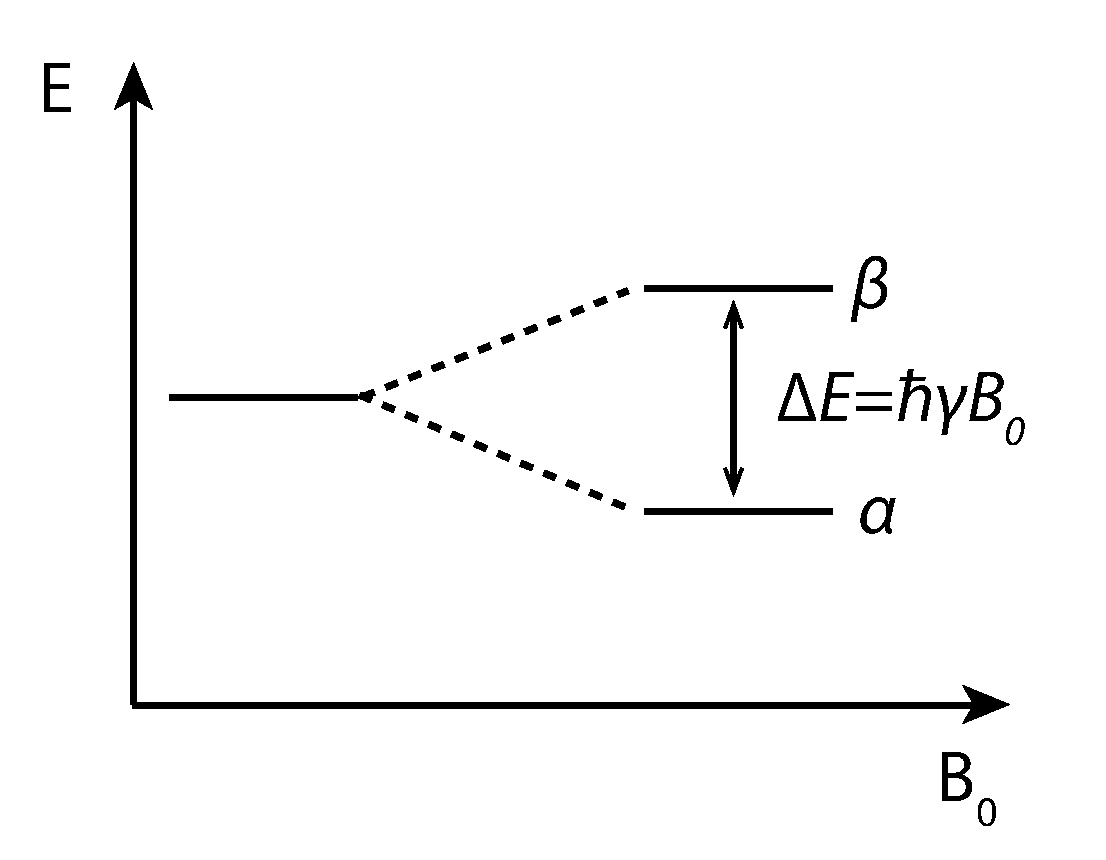
\includegraphics[width=\textwidth,height=5cm,keepaspectratio]{EigenStateLevel.pdf}
  \end{center}
  \caption{Energy level and $\Delta~E$ of the two energy levels for a spin-1/2 nucleus}
  \label{fig:EnergySplit}
\end{figure}

This splitting of energy levels due to the presence of a mganetic field is referred to as Zeeman splitting.
When examining a spin ensmeble at thermal equilibrium, overal there is a slight bias to the lower energy
state $\alpha$. This preference can be quantified by calculating the ratio of the populations, $P$:
\begin{equation}\label{eqn:Boltzmann}
  \frac{P_{\beta}}{P_{\alpha}} = \text{exp}\{\frac{-\Delta{E}}{k_B T}\}
\end{equation}
where $P_{\beta}/P_{\alpha}$ is the population ratio between the states, $k_B$ is Boltzmann constant, and $T$ is the temperature. The polarisation, $p$, of a system of
spin-1/2 nuclei is
\begin{equation}\label{eqn:Polarisation}
  p = \frac{P_\alpha - P_\beta}{P_\alpha + P_\beta}
\end{equation}

For an NMR experiment which typically operates at 298$K$ and
a field of 14.1 T the polarisation level is circa $10^{-5}$ meaning that the spins are aligned weakly
in the same direction as the magnetic field. It is this small polarisation that gives rise to the NMR
signal and why NMR is famed for sensitivity issues. One possible solution to this, hyperpolarisation, will be described in a later chapter.

When placed in a magnetic field, the nuclei will precess around the axis of the field at a rate known as the larmour frequency defined as:
\begin{equation}\label{eqn:larmor}
  \omega_j^0 = -\gamma_jB_0
\end{equation}

where $\gamma_j$ is the gyromagnetic ratio for a nucleus, $j$. The gyromagnetic ratio is
typically $10$s of MHz T$^{-1}$ that give larmour frequencies in the $100$s of MHz in an NMR
experiment.


If we let $\ket{\psi_1}$ and $\ket{\psi_2}$ be eigenstates of the Hamiltonian $\hat{\mathcal{H}}$ then
\begin{align}
  \hat{\mathcal{H}}\ket{\psi_1} = E_1\ket{\psi_1}\\
  \hat{\mathcal{H}}\ket{\psi_2} = E_2\ket{\psi_2}
\end{align}

The Hamiltonian can also be expressed in matrix form:
\begin{equation}
  \hat{\mathcal{H}} = \begin{pmatrix}
    E_1 & 0\\
    0 & E_2
\end{pmatrix}
\end{equation}
If the Hamiltonian is written in the eigenbasis of the system its main diagonal corresponds to state energies and it has values of $0$ everywhere else.

The evolution in time of a quantum system is described by the Schr\"odinger equation:
\begin{equation}
  \frac{d}{dt}\ket{\psi} = i\hbar^{-1}\hat{\mathcal{H}}\ket{\psi}
\end{equation}
the factor of $\hbar^{-1}$ here is cumbersome and can be removed by defining a Hamiltonian in natural units, $\hat{H}$
such that:
\begin{equation}
  \hat{H} = \hbar^{-1}\hat{\mathcal{H}}
\end{equation}
both Hamiltonians share the same eigenfunctions
\begin{equation}
  \hat{H}\ket{\psi_1} = \omega_{\psi1}\ket{\psi}
\end{equation}
eigenvalues are denoted $\omega_{\psi}$ and are given by:
\begin{equation}
  \omega_{\psi1} = \hbar^{-1}E_1
\end{equation}

the eiegenvalue, $\omega_{\psi1}$, is the energy of the state $\ket{\psi}$ in \textit{units} of $\hbar$.

Returning to the example of a spin-1/2 particle in a magnetic field. The Hamiltonian is initially
proportional to the $z$ angular momentum operator
\begin{equation}
  \hat{H} = \omega^0\hat{I}_z
\end{equation}

where $\omega^0 = -\gamma B_0$ and is the Larmor frequency from \eqn{eqn:larmor}. In matrix form, in the original zeeman basis, the Hamiltonian is:
\begin{equation}
  \hat{H} = \begin{pmatrix}
+\frac{\omega}{2} & 0\\
0 & -\frac{\omega}{2}
\end{pmatrix}
\end{equation}
where
\begin{equation}
  \hat{H}\ket{\alpha} = +\frac{\omega}{2}\ket{\alpha}
\end{equation}

\subsection{Spin precession}

 As discussed when describing Larmor frequency when a spin-1/2 particle is placed in
 a magnetic field it precesses at the Larmor frequency. In quantum mechanics this precession
 means that the spin state $\ket{\psi}$ depends on time.

 The law of motion for the spin is the time depenent Schr\"odinger equation:
 \begin{equation}
   \frac{d}{dt}\ket{\psi}(t) = -i\hat{H}\ket{\psi}(t)
 \end{equation}

  The spin Hamiltonian is:
  \begin{equation}
    \hat{H} = \omega^0\hta{I}_z
  \end{equation}
the equaiton of motion then becomes:
\begin{equation}
  \frac{d}{dt}\ket{\psi}(t) = -i\omega^0\hat{I}_z\ket{\psi}(t)
\end{equation}
this is a first order differential equation that has the solution:
\begin{equation}
  \ket{\psi}(t) = \text{exp}\{-i\omega^0\Delta{t}\hat{I}_z\}{\psi}(t_0)
\end{equation}
where $t_0$ is the initial time and $\Delta{t}$ is the difference in time
between $t_0$ and $t$. As the $\omega^0\Delta{t}$ term is angular fequency multiplied by
time this simply gives an angle. This shows that it is equal to a rotation about the $z$-axis:
\begin{equation}
  \hat{R}_z{\theta} = \text{exp}\{-i\theta\hat{I}_z\}
\end{equation}

The solutiuon therefore to the Schr\"odinger equation in the absence of rf fields is:
\begin{equation}
  \ket{\psi}(t) = \hat{R}_z(\omega^0\Delta{t})\ket{psi}(t_0)
\end{equation}

In the absence of r.f. fields the Schr\"odinger equation says that the spin rotates
around the $z$-axis, through the angle $\omega_0\Delta{t}$

\subsection{Rotating Frame}

The field, $B_0$, of a regular NMR experiment is many Tesla, giving precession
frequencies of hundreds of megahertz. These frequencies correspond to radio frequencies
in the electromagnetic spectrum. When considering these precessing spins
it can be useful to change from a static frame to a rotating frame of reference.

the static frame of reference axes ($x$, $y$, and $z$) and the rotating frame axes ($x'$, $y'$, and $z'$) of reference are connected through
a time dependent angle , $\Phi$(t) such that:
\begin{align}
  x' =& x\cos\Phi(t) + y\sin\Phi(t)\\
  y' =& y\cos\Phi(t) - x\sin\Phi(t)\\
  z' =& z
\end{align}
The frame rotates with a constant frequency $\omega_\text{ref}$ around the $z$-axis:
\begin{equation}
  \Phi(t) = \omega_\text{ref}t + \phi_\text{ref}
\end{equation}
for brevity $(t)$ is now dropped

If a spin in state $\ket{\psi}$ has a larmor frequency equal to $\omega_\text{ref}$
then the spin state in the rotating frame, $\ket{\tilde{\psi}}$ is:
\begin{equation}
  \ket{\tilde{\psi}} = \hat{R}_z(-\Phi)\ket{\psi}
\end{equation}
where the tilde denotes a state in the rotating frame.

These of course have an equation of motion:
\begin{equation}
  \frac{d}{dt}\ket{\tilde{\psi}} = i\hbar^{-1}\hat{\tilde{H}}\ket{\tilde{\psi}}
\end{equation}
where:
\begin{equation}\label{eqn:RotFrame}
  \hat{\tilde{H}} = \hat{R}_z(-\Phi)\hat{H}\hat{R}_z(\Phi) - \omega_\text{ref}\hat{I}_z
\end{equation}

\subsubsection{Precession in the rotating frame}
The spin Hamiltonian in a static field is:
\begin{equation}
  \hat{H}^0 = \omega^0\hat{I}_z
\end{equation}

The rotating fram Hamiltonian is:
\begin{equation}
  \hat{\tilde{H}} = \omega^0\hat{R}_z(-\Phi)\hat{I}_z\hat{R}_z(\Phi) - \omega_\text{ref}\hat{I}_z =
  (\omega^0 - \omega_\text{ref})\hat{I}_z
\end{equation}
The frequency $\omega^0 - \omega_\text{ref}$ is the differenc bwtween the larmor frequency
and that of the frame and is denoted, $\Omega^0$:
\begin{equation}
  \Omega^0 = \omega^0 - \omega_\text{ref}
\end{equation}

The rotating-frame spin Hamiltonian in the presence pf a static field, is therefore:
\begin{equation}
  \hat{\tilde{H}} = \Omega^0\hat{I}_z
\end{equation}

\subsection{Radio Frequency Pulses}

In NMR 'pulses' are used to manipulate the spin states. These pulses take the form
of an oscillating magnetic field applied at a frequency such that it is resonant with
the precessing spin. The frequencies correspond to radio frequncies anf the pulses and
fields are reffered to as r.f. pulses and r.f. fields.

When an r.f. pulse is applied, the spin experiences two magnetic fields: a static field generated
by the magnet; and an oscillating field from the excitation coil. The static field is much larger
than the oscillating r.f. field.

The weak r.f. field produces a large effect on the nuclear spin due to it being \textit{resonant}
with the precession of that spin. This allows the effect of the weak r.f. field to accumulate
as time goes on. If the pulse is applied for long enough, then the weak r.f. field can casue a
large change in the spin state. In practice, this corresponds to applying several microseconds
of an r.f. pulse which allows for several hundred Larmor precession cycles.

For an r.f. pulse of of phase, $\phi_p$, applied along the $x$-axis, the r.f. field oscillates at the spectrometer resonance frequency,$\omega_{\text{ref}}$, and  the spin Hamiltonian
during the r.f. pulse is given by:
\begin{equation}
  \hat{H} = \omega^0\hat{I}_z + \hat{H}_{\text{RF}}{t}
\end{equation}
where
\begin{equation}
  \hat{H}_{\text{RF}}(t) = -\frac{1}{2}\gamma{B_{\text{RF}}}\sin{\theta_{\text{RF}}}\hat{R}_z(\Phi_p)\hat{I}_x\hat{R}_z(-\Phi_p)
\end{equation}
and
\begin{equation}
  \Phi_p(t) = \omega_{\text{ref}}t + \phi_p
\end{equation}

The rotating frame Hamiltonian is:
\begin{align}
  \hat{\tilde{H}} =& -\frac{1}{2}\gamma{B_{\text{RF}}}\sin{\theta_{\text{RF}}}\hat{R}_z(-\Phi  +  \Phi_p)\hat{I}_x\hat{R}_z(\Phi-\Phi_p) + (\omega^0 - \omega_\text{ref})\hat{I}_z \\
  =& -\frac{1}{2}\gamma{B_{\text{RF}}}\sin{\theta_{\text{RF}}}\hat{R}_z(-\phi_{\text{ref}}  +  \phi_p)\hat{I}_x\hat{R}_z(\phi_{\text{ref}}-\phi_p) + \Omega^0\hat{I}_z
\end{align}
an additional simplification is possible if we include the value of $\phi_{\text{ref}}$ which is
$\pi$ for positive $\gamma$ spins and has the effect of changing the sign of the $\gamma{B_{\text{RF}}}$
term:
\begin{equation}
  \hat{\tilde{H}} = \omega_{\text{nut}}\hat{R}_z(\phi_p)\hat{I}_x\hat{R}_z(-\phi_p) + \Omega^0\hat{I}_z
\end{equation}
where $\omega_{\text{nut}}$ is the nutation frequency:
\begin{equation}
  \omega_{\text{nut}} = |-\frac{1}{2}\gamma{B_{\text{RF}}}\sin{\theta_{\text{RF}}}|
\end{equation}
the nutation frequency is the measure of the r.f. field amplitude.

Using the sandwhich property again the final form of the rotating-frame Hamiltonian during an r.f. pulse
is:
\begin{equation}
  \hat{\tilde{H}} = \Omega^0\hat{I}_z + \omega_{\text{nut}}(\hat{I}_x\cos\phi_p + \hat{I}y\sin\phi_p)
\end{equation}


\subsubsection{$x$-pulse}

To illustrate the effect an r.f. pulse has on a sample we consider a strong
pulse with frequency $\omega_\text{ref}$, duration $\tau$, and phase $\phi_p = 0$ (an '$x$-pulse').
The amplitude is given by $\omega_\text{ref}$. We assume this pulse to be applied
directly on resonance such that $\Omega^0 = 0$.

The rotating frame spin Hamiltonian is:
\begin{equation}
  \hat{\tilde{H}} = \omega_{\text{ref}}\hat{I}_x
\end{equation}
the motion of the spin states may be found using the rotating frame Schr\"odinger equation. If the
spin state before the pulse is given by $\ket{\tilde{\psi}}_1$ and the spin state after the pulse
is $\ket{\tilde{\psi}}_2$ then they are related by:
\begin{equation}
  \ket{\tilde{\psi}}_2 = \hat{R}_x(\theta)\ket{\tilde{\psi}}_1
\end{equation}
where the rotation operator is as defined in \eqn{eqn:RotOp} and the angle
$\theta$ is given by
\begin{equation}
  \theta = \omega_\text{nut}\tau
\end{equation}
this angle is referred to as the \textit{flip angle} of the pulse.

To calculate what effect the pulse has on spins in specific states we can use the matrix representation.
A $(\pi/2)_x$ pulse, which means a flip angle of $\theta = \pi/2$ and a phase of $\phi_p = 0$, applied to spin in the state $\ket{\alpha}$ can be calculated using the matrix representation of $\hat{R}_x(\theta)$  as:
\begin{align}
  \hat{R}_x(\pi/2)\ket{\alpha} =& \frac{1}{\sqrt{2}}\begin{pmatrix}
     \cos(\frac{1}{2}\pi/2) & -i\sin(\frac{1}{2}\pi/2)\\
     -i\sin(\frac{1}{2}\pi/2) & \cos(\frac{1}{2}\pi/2)
\end{pmatrix}\begin{pmatrix}
  1\\
  0
\end{pmatrix}\\ =& \frac{1}{\sqrt{2}}\begin{pmatrix}
  1 & -i\\
  -i & 1
\end{pmatrix}\begin{pmatrix}
  1\\
  0
\end{pmatrix}\\ =& \frac{1}{\sqrt{2}}\begin{pmatrix}
  1\\
  -i
\end{pmatrix} = e^{-i\pi/4}\frac{1}{2}\begin{pmatrix}
  1+i\\
  1-i
\end{pmatrix} = e^{i\pi/4}\ket{-y}
\end{align}
The pulse transforms the state $\ket{\alpha}$ into the state $\ket{-y}$ in other words
it has rotated the polarization by $\pi/2$ around the $x$-axis.


\subsubsection{Pulse of general phase}

To understand the significance of the phase of a pulse, consider a pulse exactly on resonance
($\Omega^0 = 0$) with a genral phase $\phi_p$. The rotating fram spin Hamiltonian is:
\begin{equation}
  \hat{\tilde{H}} = \omega_{\text{nut}}(\hat{I}_x\cos\phi_p + \hat{I}_y\sin\phi_p)
\end{equation}
from this, one can see that the effect of the phase shift is to change the axis about
which the spin polarizations rotate. The rotation axis is still in the $xy$-plane but forms
an angle, $\phi_p$, with the $x$ axis. Therefore, a pulse with a phase of $\pi/2$ rotates the spin
polarization around the $y$-axis and a phase of $\pi$ rotates the polarization around the $-x$-axis and
so on.

The propagator for an on resonance pulse with phase $\phi_p$ is given by:
\begin{align}
  \hat{R}_{\phi_p}(\theta) =& \text{exp}\{-i\omega_{\text{nut}}\tau(\hat{I}_x\cos\phi_p + \hat{I}_y\sin\phi_p)\}\\
  =& \text{exp}\{-i\theta(\hat{I}_x\cos\phi_p + \hat{I}_y\sin\phi_p)\}
\end{align}

this can be rewritten using rotation operators:
\begin{equation}
  \hat{R}_{\phi_p}(\theta) = \hat{R}_z(\phi_p)\hat{R}_x(\theta)\hat{R}_z(-\phi_p)
\end{equation}
The matrix representation can be optained by multiplying togther the matrix
representations of the rotation operators from \eqn{RotMat}:
\begin{equation}
  \hat{R}_{\phi_p}(\theta) = \begin{pmatrix}
    \cos\frac{1}{2}\theta & -i\sin\frac{1}{2}(\theta)e^{-i\phi_p}\\
    -i\sin\frac{1}{2}(\theta)e^{+i\phi_p} & \cos\frac{1}{2}\theta
\end{pmatrix}
\end{equation}

\subsubsection{Off-resonance effects}

In general, it is not always possible to ensure exact resonance for all spins at the same
time, so the condition $\Omega^0 = 0$ cannot always be satisfied. We can consider the
case when $\Omega^0 \neq 0$ by examining the spin Hamiltonian during a rectangular
pulse where:
\begin{equation}
  \hat{\tilde{H}} = \Omega^0\hat{I}_z + \omega_{\text{nut}}(\hat{I}_x\cos\phi_p + \hat{I}_y\sin\phi_p)
\end{equation}
The rotation axis of the spin polarization now has a $z$-component aswell as an $x$- and $y$-component. The
axis is therefore tilted out of the $xy$-plane.

The rotating frame spin Hamiltonian for an off-resonance pulse may be written as:
\begin{equation}
  \hat{\tilde{H}} = \boldsymbol{\omega}_{\text{eff}}\cdot\hat{\mathbf{I}}
\end{equation}
where $\boldsymbol{\omega}_{\text{eff}}$ is the effective rotation axis, given by:
\begin{equation}
  \boldsymbol{\omega}_{\text{eff}} = \omega_{\text{eff}}\{\mathbf{e}_x'\sin\beta_p\cos\phi_p + \mathbf{e}_y'\sin\beta_p\sin\phi_p + \mathbf{e}_z'\cos\beta_p\}
\end{equation}
and $\{\mathbf{e}_x',\mathbf{e}_x',\mathbf{e}_x'\}$ are the rotating reference frame axes. The vector operator
$\hat{\mathbf{I}}$ is defined as:
\begin{equation}
  \hat{\mathbf{I}} = \mathbf{e}_x'\hat{I}_x + \mathbf{e}_y'\hat{I}_y + \mathbf{e}_z'\hat{I}_z
\end{equation}
The tilt of the rotation axis away from the $z$-axis is:
\begin{equation}
  \beta_p = \arctan(\frac{\omega_{\text{nut}}}{\Omega^0})
\end{equation}
the magnitude of the rotation frequency around the tilted axis is given by:
\begin{equation}
  \omega_{\text{eff}} = \{(\omega_{\text{nut}})^2 + (\Omega^0)^2\}^{1/2}
\end{equation}
Using these parameters the rotating frame spin Hamiltonian may be written as:
\begin{equation}
  \hat{\tilde{H}} = \omega_{\text{eff}}\hat{R}_z(\phi_p)\hat{R}_y(\beta_p)\hat{I}_z\hat{R}_y(-\beta_p)\hat{R}_z(-\phi_p)
\end{equation}

The rotating-frame spin states before and after the pulse are related through:
\begin{equation}
  \ket{\tilde{\psi}}_2 = \hat{R}_{\text{off}}\ket{\tilde{\psi}}_1
\end{equation}
where $\hat{R}_{\text{off}}$ is:
\begin{equation}
  \hat{R}_{\text{off}} = \hat{R}_z(\phi_p)\hat{R}_y(\beta_p)\hat{R}_z(\omega_{\text{eff}}\tau)\hat{R}_y(-\beta_p)\hat{R}_z(-\phi_p)
\end{equation}

\subsection{The Density operator revisited}

Usually in NMR there are $>10^{20}$ spins in the sample, the density operator becomes more advantageous here
as mentioned it contains information about the entire spin ensemble. Normally, there is only a small population difference between $\alpha$ and $\beta$
governed by the Boltzmann distribution,
so for a general polarisation level, $p$, the density operator can be written as:
\begin{equation}
  \hat\rho = \frac{1}{2}\begin{pmatrix}
    1 + p & 0\\
    0 & 1 - p
\end{pmatrix}
\end{equation}
using the definition given in \eqn{eqn:operators} we can re-write this as
\begin{equation}
  \hat\rho = \frac{1}{2}\hat{\mathbb{1}} + \frac{1}{2}p\hat{I}_z
\end{equation}
$\hat{\mathbb{1}}$ is identity matrix and corresponds to no population difference between $\ket{\alpha}$ and $\ket{\beta}$.

$\hat{\mathbb{1}}$ is unaffected by rotations so can be ignored in the context of NMR
and so we write
\begin{equation}
  \hat{\rho} = \frac{1}{2}p\hat{I}_z
\end{equation}
to describe the $z$ magnetisation of our sample. If the system is at thermal equilibrium
then $p$ is equal to the Boltzmann factor defined as:
\begin{equation}
  \mathbb{B} = \frac{\hbar\gamma\B_0}{k_bT}
\end{equation}


In NMR we can  describe the dynamics of a system using the density operator evolution rather than the evolution of the states using
\begin{align}
  \frac{\partial}{\partial{t}}\ket{\psi} = -i\hat{H}\ket{\psi}\\
  \frac{\partial}{\partial{t}}\bra{\psi} = i\bra{\psi}\hat{H}
\end{align}

we can derive\citep{Neumann2018}:
\begin{align}
  \frac{\partial}{\partial{t}}\hat\rho\quad=&\quad \frac{\partial}{\partial{t}}[\ket{\psi}\bra{\psi}]\\
  =&\quad[\frac{\partial}{\partial{t}}\ket{\psi}]\bra{\psi} + \ket{\psi}[\frac{\partial}{\partial{t}}\bra{\psi}]\\
  =&\quad-i\hat{H}\ket{\psi}\bra{\psi} + i\ket{\psi}\bra{\psi}
\end{align}
to give the relationship
\begin{equation}
  \frac{\partial}{\partial{t}}\hat\rho = -i[\hat{H},\hat\rho]
\end{equation}
this is called the Liouville von Neumann equation.

The calculation of the response of the spin ensemble to r.f. pulses given the
general rotating fram as before the rotating frame density operator is given by:
\begin{equation}
  \hat{\tilde{\rho}} = \overbar{\ket{\tilde{\psi}}\bar{\tilde{\psi}}}
\end{equation}
The rotating frame and fixed frame populations and coherences are related by:
\begin{align}\label{eqn:DensityRotFrame}
  \tilde{\rho_\alpha} =& \rho_\alpha  \qquad \tilde{\rho_\beta} =& \rho_\beta\\
  \tilde{\rho_-} =& \rho_-\text{exp}\{-i\Phi(t)\} \qquad \tilde{\rho_-} =& \rho_-\text{exp}\{+i\Phi(t)\}
\end{align}
where
\begin{equation}
  \Phi(t) = \omega_{\text{ref}}t + \phi_{\text{ref}}
\end{equation}
the populations remain the same and the coherences are linked through a time dependant phase factor.

\subsubsection{Magnetization vector}

The state of a single spin-1/2 can be represented by an arrow indicating the direction of well-defined angular momentum and
the response measured by rotating the arrow around the different axes in three dimensional space. Then similarly
an ensemble of isolated spins-1/2 can be represented as a magnetization vector, $\mathbf{M}$, idicating the magnitude
and direction of the net magnetisation. The dynamics of the ensemble corresponds to the motion of the magentization vector.

The magnetization vector has three Cartesian components:
\begin{equation}
  \mathbf{M} = M_x\mathbf{e}_x + M_y\mathbf{e}_y + M_z\mathbf{e}_z
\end{equation}
 The longitudinal component is related to the population difference between states:
 \begin{equation}
   M_z = 2\mathbb{B}^{-1}(\rho_\alpha - \rho_\beta)
 \end{equation}
The transverse magnetization components $M_x$ and $M_y$ are related to the $(-1)$-quantum coherence between the states:
\begin{align}
  M_x =& 4\mathbb{B}^-1Re\{\rho_-\}\\
  M_y =& 4\mathbb{B}^-1Im\{\rho_-\}
\end{align}
These are chosen so that thermal equilibrium magnetization is a unit vector
aliong the $z$-axis:
\begin{equation}
  \mathbf{M}^{\text{eq}} = \mathbf{e}_z
\end{equation}
With these, the density operator may be written as:
\begin{align}
  \hat{\rho} =& \frac{1}{2}\mathbb{1} + \frac{1}{2}\mathbb{B}\mathbf{M}\cdot{I}\\
  =& \frac{1}{2}\mathbb{1} + \frac{1}{2}\mathbb{B}(M_x\hat{I}_x + M_y\hat{I}_y + M_z\hat{I}_z)
\end{align}
The populations and coherences can be representend in terms of magnetization:
\begin{align}
  \rho_\alpha =& \frac{1}{2} + \frac{1}{4}\mathbb{B}M_z \qquad \rho_\beta =& \frac{1}{2} - \frac{1}{4}\mathbb{B}M_z\\
  \rho_+ =&  \frac{1}{4}\mathbb{B}(M_x - iM_y) \qquad \rho_- = \frac{1}{4}\mathbb{B}(M_x + iM_y)
\end{align}

\subsubsection{Density operator under pulses}

We can use the sandwich equation to calculate the effect of a strong $(\pi/2)_x$ pulse
on an ensemble of spins-1/2 at thermal equilibrium.
Before the pulse, the spin density operator is
\begin{equation}
  \hat{\rho}_1 = \frac{1}{2}\mathbb{1} + \frac{1}{2}\mathbb{B}\hat{I}_z
\end{equation}
after the pulse the density operator is
\begin{align}
  \hat{rho}_2 =& \hat{R}_x(\pi/2)\hat{\rho}_1\hat{R}_x(-\pi/2) = \frac{1}{2}\hat{R}_x(\pi/2)\mathbb{1}\hat{R}_x(-\pi/2) + \frac{1}{2}\mathbb{B}\hat{R}_x(\pi/2)\hat{I}_z\hat{R}_x(-\pi/2) \\
  =& \frac{1}{2}\mathbb{1} + \frac{1}{2}\mathbb{B}\hat{R}_x(\pi/2)\hat{I}_z\hat{R}_x(-\pi/2)
\end{align}
since the unity matrix, $\mathbb{1}$ is invariant under rotations. The last term
can be calculated using the sandwhich relationship:
\begin{equation}
  \hat{R}_x(\pi/2)\hat{I}_z\hat{R}_x(-\pi/2) = -\hat{I}_y
\end{equation}
therefore
\begin{equation}
  \hat{\rho}_2 = \frac{1}{2}\mathbb{1} - \frac{1}{2}\mathbb{B}\hat{I}_y
\end{equation}

In terms of the magnetisation vector, this is equivalent to rotating
the magnetization from the $z$-axis to the $-y$-axis.
\begin{equation}
  \mathbf{M}_1 = \mathbf{e}_z \xrightarrow{(\pi/2)_x} mathbf{M}_2 = -\mathbf{e}_y
\end{equation}

To determine what happens to the populations and coherences we can look at the
pulse effects in terms of the matrix representation:
\begin{equation}
  \hat{\rho}_1 = \begin{pmatrix}
    \frac{1}{2} + \frac{1}{4}\mathbb{B} & 0\\
    0 & \frac{1}{2} - \frac{1}{4}\mathbb{B}
\end{pmatrix}\xrightarrow{(\pi/2)_x}\begin{pmatrix}
  \frac{1}{2} & -\frac{1}{4i}\mathbb{B}\\
  \frac{1}{4i}\mathbb{B} & \frac{1}{2}
\end{pmatrix}
\end{equation}
the pulse accomplishes two things, firstly, the pulse equalizes the populations of the
two states and secondly, converts the population difference into coherences.

\subsection{Free evolution with Relaxation}

So far, we have only discussed the Hamiltonian and density operator before, during and
immediately after an r.f. pulse. This picture is insufficient to describe what one observes
experimentally. In terms of populations and cohenrences, experimentally we find that
the populations are not time independent but gradually drift towards their thermal
equilibrium values and that the coherences do not last forever but gradually decay
to zero.

For populations and coherneces there are two forms of relaxation, $T_1$ and $T_2$. $T_1$ is the longitudal relaxation time
constant and $T_2$ is the transverse relaxation time constant. The difference between them is demonstrated in \fig{fig:t1t2}. Classically
$T_1$ is the rate constant that governs the return of magnetisation to the $z$-axis from the $xy$-plane. $T_2$ on
the other hand is the time constant that governs the return of magnetisation to equilibrium in the $xy$-plane.
When talking in terms of the density operator we say that $T_1$ is the relaxation rate constant for populations, and $T_2$ is the relaxation
rate constant coherences. But this is incompatible with the classical description of NMR.

The Bloch equations are used to describe how the megnetisation vectors change in time\ref{Bloch:1946hk}:
\begin{align}
  \frac{dM_x(t)}{dt}\quad=&\quad\gamma(M_y(t)B_z(t)-M_z(t)B_y(t)) - \frac{M_x(t)}{T_2}\\
  \frac{dM_y(t)}{dt}\quad=&\quad\gamma(M_z(t)B_x(t)-M_x(t)B_z(t)) - \frac{M_y(t)}{T_2}\\
  \frac{dM_z(t)}{dt}\quad=&\quad\gamma(M_x(t)B_y(t)-M_y(t)B_x(t)) - \frac{M_z(t)-M_0}{T_1}
\end{align}

\begin{figure}[h]
  \center{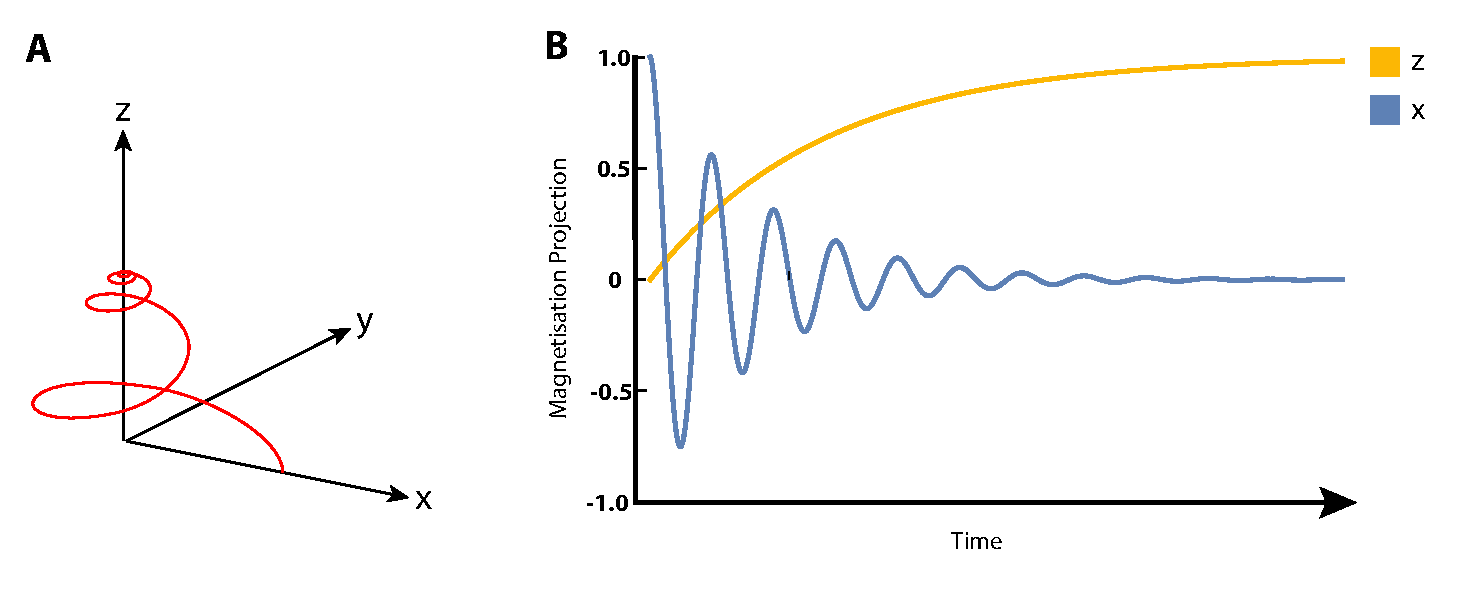
\includegraphics[width=\textwidth]{T1T2.pdf}}
  \caption{A) a magnetisation vector precesses in the $xy$-plane, eventually returning to equilibrium.
  B) A plot of the magnetisation along $z$-axis (yellow) and the $x$-axis (blue) during the relaxation.}
  \label{fig:t1t2}
\end{figure}

\subsubsection{Transverse relaxation}\label{T2}

The coherences decaying to zero is ensured in the equations by introducing an exponential decay term.
between time points $2$, immediately after an r.f. pulase, and $3$ with some delay $\tau$ the
equations for the rotating frame coherences are:
\begin{align}\label{eqn:coherencetime}
  \rho_-(3) =& \rho_-(2)\text{exp}\{(i\Omega^0 - \lambda)\tau\}\\
  \rho_+(3) =& \rho_+(2)\text{exp}\{(-i\Omega^0 - \lambda)\tau\}
\end{align}
where the damping rate constant $\lambda$ is given by the inverse of the
transverse relaxation time constat $T_2$:
\begin{equation}
  \lambda = T_2^{-1}
\end{equation}

These equations for coherences correspond to the following substitution rules
for the transverse spin angular momentum operators:
\begin{align}
  \hat{I}_x \rightarrow& (\hat{I}_x\cos\Omega^0\tau + \hat{I}_y\sin\Omega^0\tau)e^{-\lambda\tau}\\
  \hat{I}_y \rightarrow& (\hat{I}_y\cos\Omega^0\tau - \hat{I}_x\sin\Omega^0\tau)e^{-\lambda\tau}
\end{align}

For the transverse components of the magnetization vector, the equations are:
\begin{align}
  M_x(3) =& M_x(2)\cos\Omega^0\tau + M_y(2)\sin\Omega^0\tau)e^{-\lambda\tau}\\
  M_y(3) =& M_y(2)\cos\Omega^0\tau - M_x(2)\sin\Omega^0\tau)e^{-\lambda\tau}
\end{align}

Physically, coherence requires a consistent polarization direction of the spin ensemble. On
average all spins experience the same field in a liquid due to motional averaging, however, at
any particular instant in time the field are slightly different for different spins locally which
cause a gradual loss of synchronization across the ensemble. Coherence decay does increase the entropy
of the spin ensemble and is therefore irreversible.

\subsubsection{Longitudinal relaxation}

The equations of motion for the populations is a bit more complicated as the populations decay back
to their thermal equilibrium values the equations for this are:
\begin{align}
  \rho_\alpha(3) =& (\rho_\alpha(2)-\rho_\alpha^{eq})e^{-\tau/T_1} + \rho_\alpha^{eq} \\
  \rho_\beta(3) =& (\rho_\beta(2)-\rho_\beta^{eq})e^{-\tau/T_1} + \rho_\beta^{eq}
\end{align}
where the thermal equilibrium populations are:
\begin{equation}
  \rho_\alpha^{eq} = \frac{1}{2} + \frac{1}{4}\mathbb{B} \qquad \rho_\beta^{eq} = \frac{1}{2} - \frac{1}{4}\mathbb{B}
\end{equation}

The equation of motion for the $z$-axis magnetisation vector is:
\begin{equation}
  M_z(3) = (M_z(2) - 1)e^{-\tau/T_1} + 1
\end{equation}

Longitudinal relaxation involves an energy exchange between the spin system and the molecular
surroundings and is why it is often referred to as spin-lattice relaxation.

\Subsection{NMR signal and detection}

In NMR the signal produced by the spins is inductively detected. The precessing transverse magnetization, created
when an r.f. field is applied to the sample, induces a voltage, and therefore a current, in a coil that
is placed near the sample.

In order to do this, consider a sample containing $n_s$ number of non-interacting spins-1/2 which have a
sample volume, $V_s$, and a concentration of spins, $c_s$.
The total magnetic dipole moment operator in this case is:
\begin{equation}\label{eqn:MagneticMoment}
  \hat{\boldsymbol{\mu}} = \hbar\gamma\sum_{k=1}^n\mathbf{\hat{I}}_k
\end{equation}
where $\mathbf{\hat{I}}_k$ is the spin angular momentum operator for a nucleus $k$ such that:
\begin{equation}
  \mathbf{\hat{I}}_k = (\hat{I}_{kx}\mathbf{e}_x + \hat{I}_{ky}\mathbf{e}_y + \hat{I}_{kz}\mathbf{e}_z)
\end{equation}

The total magnetisation of the sample is given by:
\begin{equation}\label{eqn:magnetization}
  \mathbf{M} = \frac{\sum_{k=1}^n\hat{\boldsymbol{\mu}}}{V_s} = \frac{c_sV_s\langle\overbar{\boldsymbol{\mu}}\rangle}{V_s} = c_s\langle\overbar{\hat{\boldsymbol{\mu}}}\rangle
\end{equation}
where $\langle\overbar{\hat{\boldsymbol{\mu}}}\rangle$ is the ensemble average magnetic dipole moment for the sample.

This magnetisation leads to the signal obtained in NMR, to find the relationship we can
invoke the principle of reciprocity \citep{Hoult:1976dw}. Consider the induction
field, $mathbf{B}_1$, produced by a coil carrying unit current. For a magnetic dipole, $\mathbf{m}$,
the induced emf is given by:
\begin{equation}
  \xi = -\frac{\partial}{\partial{t}}\{\mathbf{B}_1\cdot\mathbf{m}\}
\end{equation}
where $\mathbf{B}_1$ is the field produced by the unit current in the wire at $\mathbf{m}$. It follows
that for our sample after being subjected to a $(\pi/2)$ pulse, we need only know the value of
$\mathbf{B}_1$ at all points within the sample to be able to calculate the emf induced
in the coil if $\mathbf{M}$ lies in the $xy$-plane:
\begin{equation}
  \xi = -\int_{\text{sample}} \frac{\partial}{\partial{t}}\{\mathbf{B}_1\cdot\mathbf{M}\} dV_s
\end{equation}
as $\mathbf{B}_1$ is considered to be homogeneous over the sample volume this gives:
\begin{equation}
  \xi = \frac{\partial}{\partial{t}}\{\mathbf{B}_1\cdot\mathbf{M}\}V_s
\end{equation}
we can sub in the result from \eqn{eqn:magnetization} to give
\begin{equation}
  \xi = \frac{\partial}{\partial{t}}\{\mathbf{B}_1\cdot\langle\overbar{\hat{\boldsymbol{\mu}}}\rangle\}V_sc_s
\end{equation}
if we take the $B_1$ coil to be aligned along the $x$-axis, the $x$-axis components contribute to the emf
\begin{equation}
  \xi = \frac{\partial}{\partial{t}}\{B_{1x}\langle\overbar{\hat{\mu}}_x\rangle\}V_sc_s
\end{equation}
using \eqn{eqn:MagneticMoment} we get that $\langle\hat{\mu}_x\rangle = \hbar\gamma\langle{\hat{I}_x}\rangle$
the emf becomes
\begin{equation}
  \xi = \frac{\partial}{\partial{t}}\{B_{1x}\langle\overbar{\hat{I}_x}\rangle\}V_sc_s\hbar\gamma
\end{equation}
form \ref{Density} we find that the ensemble average can be found using the density operator
$\langle{\hat{I}_x}\rangle = \text{Tr}\{\hat{\rho}\hat{I}_x\}$ so
\begin{align}
  \xi = \frac{\partial}{\partial{t}}\{B_{1x}[\text{Tr}\{\hat{\rho}\hat{I}_x\}]\}V_sc_s\hbar\gamma
  \xi = \frac{\partial}{\partial{t}}\{B_{1x}[\rho_- + \rho_+]\}V_sc_s\hbar\gamma\frac{1}{2}
\end{align}
all terms apart from the coherences are time independent so the emf can be simplified for now as
\begin{equation}
  \xi \~ \frac{\partial}{\partial{t}}\rho_-(t) + \frac{\partial}{\partial{t}}\rho_+(t)
\end{equation}
using \eqn{eqn:coherencetime}
\begin{align}
  \rho_-(t) =& \rho_-(0)\text{exp}\{(i\omega^0-\lamba)t\}\\
  \rho_+(t) =& \rho_-(0)\text{exp}\{(-i\omega^0-\lamba)t\}
\end{align}
the emf becomes
\begin{equation}
  \xi \~ (i\omega^0\rho_- - i\omega^0\rho_+)
\end{equation}

the signal that one obtains in an NMR experiment is proportional to the emf induced in the pick-up coil this
is denoted $s_\text{FID}$ and is given by:
\begin{equation}
  s_\text{FID} ~ (i\omega^0\rho_- - i\omega^0\rho_+)\frac{1}{2}\frac{B_1}{i}\gamma\hbar~c_sV_s
\end{equation}

\subsubsection{Quadrature detection}

This 'raw' NMR signal oscialltes at many hundred megahertz which is too fast for
conversion to a digital signal that can be interpeted on a computer. Therefore,
it is neccesary to down convert the frequency of the NMR signals. This is accomplished
by subtracting a frequency that is close to the Larmor frequency, typically, the frequency
we subtract is set somewhere in the middle of the spectrum. This frequency is usually generated locally
by an r.f. synthesizer and is called the reference fequency and denoted $\omega_\text{ref}$ and has an associated
phase $\phi_\text{ref}$

This process of subtraction is carried out by a device called a mixer. The mixer
achieves this by multiplying together the two input signals. The signal from the FID is
multiplied by the receiver reference signal:
\begin{equation}
  s_{\text{rec}}(t) = \cos(\omega_{\text{ref}}t + \phi_{\text{rec}})
\end{equation}
the reference signal is split into two parts $A$ and $B$ where $A$ has the same form as above and $B$ is
given an additional phase shift so:
\begin{align}
  s_{\text{rec}}^A(t) =& \cos(\omega_{\text{ref}}t + \phi_{\text{rec}})\\
  s_{\text{rec}}^B(t) =& \cos(\omega_{\text{ref}}t + \phi_{\text{rec}} + \pi/2)
\end{align}

The signal after mixing with $A$ is:
\begin{equation}
  s_{\text{FID}}(t)s_{\text{rec}}^A(t) = (i\omega^0\rho_-(t) - i\omega^0\rho_+(t))\cos(\omega_{\text{ref}}t + \phi_{\text{rec}})
\end{equation}
which can be evaluated as
\begin{align}
  s_{\text{FID}}(t)s_{\text{rec}}^A(t) =& \frac{1}{2}i\rho_-(0)\text{exp}\{i[(\omega^0 + \omega_{\text{ref}})t + \phi_{\text{rec}}]\}e^{-\lamba)t}\\
                                        &+\frac{1}{2}i\rho_-(0)\text{exp}\{i[(\omega^0 - \omega_{\text{ref}})t - \phi_{\text{rec}}]\}e^{-\lamba)t}\\
                                        &-\frac{1}{2}i\rho_+(0)\text{exp}\{i[-(\omega^0 - \omega_{\text{ref}})t + \phi_{\text{rec}}]\}e^{-\lamba)t}\\
                                        &+\frac{1}{2}i\rho_+(0)\text{exp}\{i[-(\omega^0 + \omega_{\text{ref}})t - \phi_{\text{rec}}]\}e^{-\lamba)t}
\end{align}
This rather complicated signal is now passed through a low pass r.f. filter which removes the high frequncy components this
removes the components oscillating at $\omega^0 + \omega_{\text{ref}}$ and retains the low frequency components
$\Omega^0 = \omega^0 - \omega_{\text{ref}}$ the signal $s_A(t)$ emerging from the filter is
\begin{align}
  s_A =& +\frac{1}{2}i\rho_-(0)\text{exp}\{i(\Omega^0t - \phi_{\text{rec}})\}e^{-\lamba)t}\\
       & -\frac{1}{2}i\rho_+(0)\text{exp}\{i(-\Omega^0t+ \phi_{\text{rec}})\}e^{-\lamba)t}
\end{align}
due to the relationship between labratory and rotating-frame coherences from \eqn{eqn:DensityRotFrame}
this can be written as
\begin{align}
  s_A =& +\frac{1}{2}i\tilde{\rho}_-(0)\text{exp}\{i(\Omega^0t - \phi_{\text{rec}} + \phi_{\text{ref}})\}e^{-\lamba)t}\\
       & -\frac{1}{2}i\tilde{\rho}_+(0)\text{exp}\{i(-\Omega^0t+ \phi_{\text{rec}} - \phi_{\text{ref}})\}e^{-\lamba)t}
\end{align}
where $\phi_{\text{ref}}$ represents the angle of the rotating frame with respect to the labratory frame
at time $t = 0$. The equations for the precession in the rotating from (\eqn{eqn:coherencetime})
allow for the simplification
\begin{equation}
  s_A = +\frac{1}{2}i\tilde{\rho}_-(t)\text{exp}\{-i(\phi_{\text{rec}} - \phi_{\text{ref}})\}
        -\frac{1}{2}i\tilde{\rho}_+(t)\text{exp}\{i(\phi_{\text{rec}} - \phi_{\text{ref}})\}
\end{equation}
The same arguments can be repeated for the phase shifted signal path $B$
\begin{equation}
  s_B = +\frac{1}{2}\tilde{\rho}_-(t)\text{exp}\{-i(\phi_{\text{rec}} - \phi_{\text{ref}})\}
        +\frac{1}{2}\tilde{\rho}_+(t)\text{exp}\{i(\phi_{\text{rec}} - \phi_{\text{ref}})\}
\end{equation}

These signals are treated as two components of one complex signal:
\begin{equation}
  s(t) = s_A(t) + is_B(t)
\end{equation}
which evaluates to
\begin{equation}
  s(t) \~ i\tilde{\rho}_-(t)\text{exp}\{-i(\phi_{\text{rec}} - \phi_{\text{ref}})\}
\end{equation}
Which contains contributions from the rotating frame ($-1$)-quantum coherences. The ($+1$)-quantum coherences
have disappeared however, the contribution is equal to the ($-1$)-quantum coherence so a factor two is included
the frame phase shift as well as other sources of constant shifts from instrumentation are corrected in post-processing
so the quadrature signal can be expressed as:
\begin{equation}
  s(t) \~ 2i\tilde{\rho}_-(t)\text{exp}\{-i\phi_{\text{rec}}\}
\end{equation}
There are some time independant variables from the original expression of $s_{\text{FID}}$ which can now be included:
\begin{align}
  s(t) =& 2i\omega^0\frac{1}{2}\frac{B_{1x}}{i_c}\gamma\hbar~c_sV_s\tilde{\rho}_-(t)\text{exp}\{-i\phi_{\text{rec}}\}\\
  s(t) =& i\omega^0\frac{B_{1x}}{i_c}\gamma\hbar~c_sV_s\tilde{\rho}_-(t)\text{exp}\{-i\phi_{\text{rec}}\}
\end{align}
where $\omega^0$ is the larmor frequency, $\frac{B_{1x}}{i_c}$ is the coil sensitivity, $\gamma$ is the gyromagnetic ratio,
$\hbar$ is the reduced Planck's constant, the term $c_sV_s$ is the number of spins in the sample. This signal is still
strictly speaking a voltage that produces an osciallting current

\subsubsection{Signal after a pulse}


The signal dependence can be seen more clearly if one gets more quantitative, to do this,
consider a $(\pi/2)_x$ pulse with receiver phase, $\phi_{\text{rec}} = 0$, for brevity the
tilde will be dropped as the rotating frame will be considered. In order to calculate the $(-1)$-quantum coherence we must
first calculate the density operator. The rotating frame density operator at equilibrium is
\begin{equation}
  \hat{\rho}^{eq} = \frac{1}{2}\mathbb{1} + \frac{1}{2}\mathbb{B}\hat{I}_z
\end{equation}
immediately after the pulse at $t=0$ the density operator is
\begin{equation}
  \hat{\rho}(0) = \frac{1}{2}\mathbb{1} - \frac{1}{2}\mathbb{B}\hat{I}_y
\end{equation}
this can be written in terms of the shift and projection operators:
\begin{equation}
  \hat{\rho}(0) = \frac{1}{2}\hat{I}^{\alpha} + \frac{1}{2}\hat{I}^{\beta} - \frac{1}{4i}\mathbb{B}\hat{I}^+ + \frac{1}{4i}\mathbb{B}\hat{I}^-
\end{equation}
the $(-1)$-quantum coherence is equal to the coeffecient of the $\hat{I}^-$ operator
\begin{equation}
  \rho_-(0) = \frac{1}{4i}\mathbb{B}
\end{equation}
the coherence at a time $t>0$ is given by:
\begin{equation}
  \rho_-(t) = \rho_-(0)\text{exp}\{(i\Omega^0 -\lambda)t\}
\end{equation}

By combining this with the signal equation:
\begin{equation}
  s(t) = a \text{exp}\{(i\Omega^0 -\lambda)t\}
\end{equation}
where the signal amplitude $a$ is
\begin{equation}
  a = i\omega^0\frac{B_{1x}}{i_c}\gamma\hbar~c_sV_s\rho_-(0)\text{exp}\{-i\phi_{\text{rec}}\}
\end{equation}
and in the case of the $(\pi/2)_x$ pulse
\begin{equation}
  a = i\omega^0\frac{B_{1x}}{i_c}\gamma\hbar~c_sV_s\frac{1}{4i}\mathbb{B}
\end{equation}
collecting like terms and expanding $\mathbb{B}$ gives
\begin{equation}
  a = \frac{1}{4}\frac{B_{1x}}{i_c}\gamma^3\hbar^2\B_0^2\frac{n_s}{k_bT}
\end{equation}
where $n_s$ is the number of spins in the sample. This relationship makes sense intuitively
as increasing the number of spins in your sample leads to an increase in single amplitude as does increasing the
coil sensititivity.

\subsubsection{Fourier Transform}

After applying an r.f. pulse, the resulting free induction decay (FID) measured is typically an exponentionally decaying sinusoidal function.
The signal produced from this can be written generally as:
\begin{align}\label{eqn:signal}
  S(t) =& \sum_l s_l(t) \\
  s_l(t) =& a_l\text{exp}\{-(i\omega_l+\lambda_l)t\}
\end{align}
where $S(t)$ is the total signal from from the sample and $s_l$ are the signals from the individual spins. Each spin has an
amplitude, $a_l$, and an associated decay constant, $\lambda_l = T_2^{-1}$.

$S(t)$ is easy to evaluate and interpret if it originates from one spin or a group of spins precessing
at precisely the same frequency, however, if there are more spins in the sample processing at different frequencies
the FID becomes extremely hard to interpret on its own.

We can clear this picture up however by employing a Fourier transform. This comverts the time-domain data
into the frequncy-domain, such that the total signal in the frequency domain, $S(\Omega)$ is the sum of all individual spin signals resonating at the frequency, $S_l(\Omega)$:
\begin{equation}
  S(\Omega) = \sum_l S_l(\Omega)
\end{equation}
This allows us to clearly see which resonances are possessed by our spins in the sample. To
perform a Fourier transform we must do the following:
\begin{equation}
  S_l(\Omega) = \int_{0}^{\infty}s_l(t)\text{exp}\{-i\Omega t\}dt
\end{equation}
and using \eqn{eqn:signal} can be rewritten:
\begin{equation}
  S_l(\Omega) = a_l\int_{0}^{\infty}\text{exp}\{(-i(\Omega+\Omega_l)+\lambda_l t\}dt
\end{equation}
sometimes written more concisely as:
\begin{equation}
  S(\omega) = \mathcal{F}\{S(t)\}(\Omega)
\end{equation}
where $S(t)$ is the signal for the time domain (FID) and $S(\omega)$ is the signal in the frequency domain.

The Fourier transform of our general case is:
\begin{equation}
  \mathcal{F}\{S(t)\}(\omega) = a_l\frac{1}{\lambda_l + i(\omega - \omega_l)}
\end{equation}
which is Lorentzian function centered at $\omega_l$ with peak width parameter $\lambda_l$.

The NMR signal represented in the frequency domain is a spectrum. It is usually consists of many peaks
indicating different resonance frequencies of spins in the sample. In the next
section we will discuss chemical shift and J-coupling. Two additional effects that when combined
with larmour frequencies already discussed form the NMR spectrum as we know it.

\subsubsection{Chemical Shift and J-coupling}

In a molecule, nuclei are surrounded by clouds of electrons which can shield, or de-sheild, it
from the effects of the external field $B_0$.

The chemical shielding factor, $\sigma$, shifts the resonance frequency of the nuclear spin. We
can now include it in \eqn{eqn:larmour}:
\begin{equation}
  \omega_j^0 = -\gamma_jB_0(1-\sigma)
\end{equation}
this chemical shielding is specific to each nuclei position in the molecule. It is possible
for two or more nuclei to share the same factor. We refer to these as being chemically equivalent.

The shielding is often around $10^{-6}$ for $\ce{^1H}$, when plotting and examining spectra
it would not be useful to use absolute frequecies, as discussed they are regularly in the hundreds of MHz,
whereas the differences in peaks might only be kHz or less. To combat this we use a relative frequency scale
called chemical shift, $\delta$, defined as:
\begin{equation}
  \delta = \frac{\omega_j-\omega^\text{ref}_j}{\omega^\text{ref}_j}
\end{equation}
where $\omega_j$ is the precession frequency of the nucleus of interest, and $\omega^\text{ref}_j$ is the precession
frequency of a reference nucleus. $\delta$ is a dimentionless number, unaffected by magnetic field strength, it often
small compared to the size of the field and is reported in parts per million (ppm).

In addition to the external $B_0$ field, the nuclear spins are also affected by the magnetic fields generated
by neighboring spins. These magnetic fields are mediated by the electrons in the chemical bonds. This is refered to as
spin-spin couling or $J$-coupling and gives rise to peak splittings in spectra. These splittings, and therefore the values
of $J$-couplings, range from a few Hz to a thousand Hz typically. These become important when considering the
Hamiltonian of a multi-spin system but is not discussed in this work.

Both of these, $\sigma$ and $J$-couplings, are tensors this means they depend on the orientation of the molecule
and the spin with respect to the magetic field. In liquids, however, tumble rapidly compared to the timescale
of an NMR experiment. This averages the interactions resulting in a scalar quantity for each.

There are additional effects the nuclear spins experience, for example, dipole-dipole coupling which
is a through space spin-spin coupling, and quadrapole coupling where there are spins with >1/2 values
however, these are not relevant to this work.

\newpage

\section{Micro-NMR}\label{Micro-NMR}

All NMR experiments depend on two performance metrics: sensitivity and resolution. Sensitivity
here means the minimum number of spins needed to give a signal clearly above the noise. Resolution
quantifies how well different spins in the sample can be differentiated. These two properties
are often linked, by selecting a smaller sample it is possible to enhance resolution by detecting
a smaller portion of spins in the sample but this compromises sensitivity as the number of spins become more limited.

 In NMR, the long life time of the nuclear spin states (minutes in some cases) contirbute to extremely
 narrow lines in the spectrum with resolutions of one part per billion regularly acheived in
 commercial systems.

 \subsection{Sensitivity}

 \subsubsection{Signal to noise ratio}


 Sensitivity in NMR at thermal equilibrium is always in short supply. In an NMR experiment, the signal amplitude
 at thermal equilibrium $a$ can be expressed as:
\begin{equation}\label{eqn:Hale}
 a = \frac{1}{4}\frac{B_{1x}}{i_c}\gamma^3\hbar^2\B_0^2\frac{n_s}{k_bT}
\end{equation}
where $\gamma$ is the gyromagnetic ratio of the nucleus,$\hbar$ is Planck's constant $h/2\pi$, $B_0$ is the magnetic field, $n_s$ is
the number of spins in the sample, $k_B$ is the Boltzmann constant and $T$ is the absolute temperature. The amplitude
of the signal depends on the bolztmann distribution of population which at room temperature is on the order of $10^{-25}$J
which is much lower that the thermal energy of the system. From the equation, increasing $B_0$ would seem a
valid strategy and comparatively it can be, increasing from 14.1T to 23.5T can almost triple the signal amplitude,
however even at 23.5T there is only a factor of ~$6\times10^{-6}$ in population difference. It's this
very small value that is responsible for the low sensitivity of NMR compared to other techniques.

As mentioned, detection in NMR is typically done through the induction of a voltage in a coil that's close
to the precessing nuclear spins this is usually referred to as the sample coil. Unfortunately,
this coil also brings with it a type of interference, noise, analagous to the 'hiss' in the backgound
of radio it is produced mainly from thermal motion of electrons in the sample coil with some contribution from thermal
motion of ions in solution. The signal to noise ratio, SNR, is an important factor in NMR experiments if its too low
the signal will never be seen.

The SNR was formulated by Abragam\citep{Abragam:1961vg} and the analysis extended by Hoult and
Richards\citep{Hoult:1976dw} and is defined as the peak signal divided by the root mean square (rms) noise. By including
the amplitude from \eqn{eqn:Hale} and using the \textit{Rayleigh-Jeans approxiamation} for the noise we find:
\begin{equation}\label{eqn:SNR}
  \text{SNR} = \frac{k_0\frac{1}{4}\frac{B_{1x}}{i_c}\gamma^3\hbar^2\B_0^2\frac{n_s}{k_bT_s}}{F\sqrt{4k_bT_cR_{\text{noise}}\Delta~f}}
\end{equation}
where k_0 is a factor that accounts for inhomogeniety in the $B_1$ field, $n_s$ is the number of spins in the sample,
$\omega_0$ is the larmour frequency. The factor $B_1/i_c$ the magnetic field from the coil per unit current is defined
as the coil sensitivity. The denominator is the noise determined by the noise factor from the spectrometer ($F$) and
the dissipative loses ($R_{\text{noise}}$) of the coil, circuit and sample for the spectral bandwidth $\Delta~f$.
$T_c$ is the absolute temperature of the coil, and $k_b$ is the boltzmann constant.

In the same paper, Hoult and Richards introduced the principle of reciprocity for calculating the
sensitivity of the RF coil, This states that the signal received from a sample by a coil is proportional to the magnetic
field which would have been created in the sample if unit current were passed through the coil. Therefore the SNR is
directly proportional to the sensitivity of the coil, $B_1/i$. This can be seen if we define an
effective sample volume that is the volume in which $B_1$ is within 10\% of the maximum
value at the center of the coil. The SNR is given by a more simple expression\citep{vanBentum:2007fda}:
\begin{equation}
  SNR = C\frac{B_1n_s}{i_c\sqrt{R\Delta~f}}
\end{equation}
where $n_s$ is the number of spins in located within an effective volume.
For protons at 600MHz the constant, $C$ equals $1.4\times10^{-11}$ in SI units ($B_0$ = 14.1T, $T$ = 300K, $\gamma$ =
$0.2675\times10^9$ $\text{rad} \text{T}^{-1}\text{s}^{-1}$, $I = 1/2$ and $F = 1$ assuming neglible noise from the spectrometer.)

From the simple expression it becomes clear that the way to improve SNR is to increase the filling factor, maximise coil sensitivity,
$B_1/i_c$, and minimise the total resistance. The filling factor, $\alpha_F$ is given by:
\begin{equation}\label{eqn:FillingFactor}
  \alpha_F = \frac{\int~B_1^2\rho(r)dV}{\int~B_1^2dV}
\end{equation}
where the function $\rho$ is unity in the sample area, and zero elsewhere. For a long solenoid coil with the
interior space filled with sample, $\alpha_F = 1/2$.

Increasing the filling factor and maximising maximise coil sensitivity, can be solved by decreasing the size of
the detector. The third, minimising resistance in the coil
can be tackled by commercially available cryoprobes where the coil is cooled with a stream of He gas to
~20K this reduces the thermal noise from the source and can increase SNR by a factor of four.

To see how size of coil affects SNR we take an RF helical coil. An idealised coil
is a cylindrical shell with uniform current density. The RF current penetrates to a frequency
specific depth $\delta$. For copper at 600 MHz and room temperature $\delta$ = 2.7 $\mu$m. The center
field is given by:
\begin{equation}
  \frac{B_1}{i_c} = \frac{\mu_0}{\sqrt{l^2+d^2}}
\end{equation}
Resistance is:
\begin{equation}
  R = \rho_r\frac{\pi~d}{l\delta}
\end{equation}
with $l$, the height of the copper cylinder, $d$ the diameter and $\rho_r$ the resistivity.
Optimum coil sensitivity is given by $d/l$ = $1$ in this case the signal to noise is:
\begin{equation}
  SNR = 0.9\times10^{-16}\frac{N_s}{d\sqrt{\Delta~f}}
\end{equation}
For a fixed number of spins the SNR scales with 1/d as predicted by \citep{Hoult:1976dw}

\subsection{Limit of Detection}

The signal to noise ratio can be found in the time or frequency domain. In the time domain the noise, $N$, is proportional to
$\sqrt{\Delta~f}$. Therefore the SNR in the time domain is not a good measure of sensitivity, it can be
artificially inflated by narrowing the bandwidth. Instead it is better to use \textit{limit of deteciton}, deined as
the number of spins that have to resonate within a bandwidth of 1 Hz to give an SNR of 3. This gives
the normalised limit of detection as\citep{Badilita:2011td}:
\begin{equation}
  \text{nLOD}_{t} = \frac{3n_s}{\text{SNR}_{t}\sqrt{\Delta~f}}
\end{equation}
Where $n_s$ is the number of spins that were present in the sample for the measurement and $\text{SNR}_t$ is the
signal to noise ratio in the time domain.
In the frequency domain, this becomes
\begin{equation}\label{eqn:nLOD}
  \text{nLOD}_\omega = \frac{3n_s\sqrt{\Delta~t}}{\text{SNR}_\omega}
\end{equation}
here, $\Delta~t$ is the effective acquisition time for a single scan given by the inverse of the
line broadening applied in the processing of the spectrum.

Practically, NMR relies on signal averaging (see \ref{Signal Averaging}) to enhance the spectra. This
method requires waiting between scans for the spins to reach thermal equilibrium. In
this case, a better measure of sensitivity can be applied by using total measurement time
as $\Delta~t$. The drawback here, is that the limit of detection now depends on instrumentation
and sample as $T_1$ relaxation dictates the experiment repetition rate.

\subsection{Concentration limit of detection}

Both types of LOD discussed so far are absolute measures. It is often of more
interest to examine the \textit{concentration} limit of detection cLOD. This is given by
dividing the LOD by the sample volume:
\begin{equation}\label{eqn:cLOD}
  \text{cLOD} = \frac{nLOD}{V_s} =\frac{\text{nLOD}}{\alpha_fV_c}
\end{equation}
Where $V_c$ is the volume of the coil and $\alpha_f$ is the filling factor defined in \eqn{eqn:FillingFactor}.

\eqn{eqn:SNR} and \eqn{eqn:Hale} show that overall the SNR and
magnetization depend on number of spins and energy level population differences, therefore, best practice
would be to wherever possible have higher $B_0$ to increase population differences and in the case of
concentrated limited samples to have a larger volume, increasing the number of spins.
One of the major reasons, however, for development of micro-NMR has been the scaling of SNR and thefore LOD
with coil size. The trade off here is that as the coil size, and LOD, becomes lower and lower, the
volume shrinks too which leads to losses in cLOD. Micro-NMR therefore, only makes sense for mass
or volume limited samples.


\subsection{Transmission line probe}

This work employs the use of a planar transmission line probe(TLP)\citep{Finch:2016gv, RN164}, in which the geometry
differs from that of a classic micro-coil. The design of which is based off early work by van Bentum \textit{et
al.} and for an equivalent helix gives $\sqrt{2}$ larger SNR\citep{vanBentum:2007fda}. The design of the TLP is shown in
\fig{fig:MVProbe}. It works with a generic microfluidic device that has well defined outer geometry and a fixed sample
chamber position.
\begin{figure}
  \begin{center}
  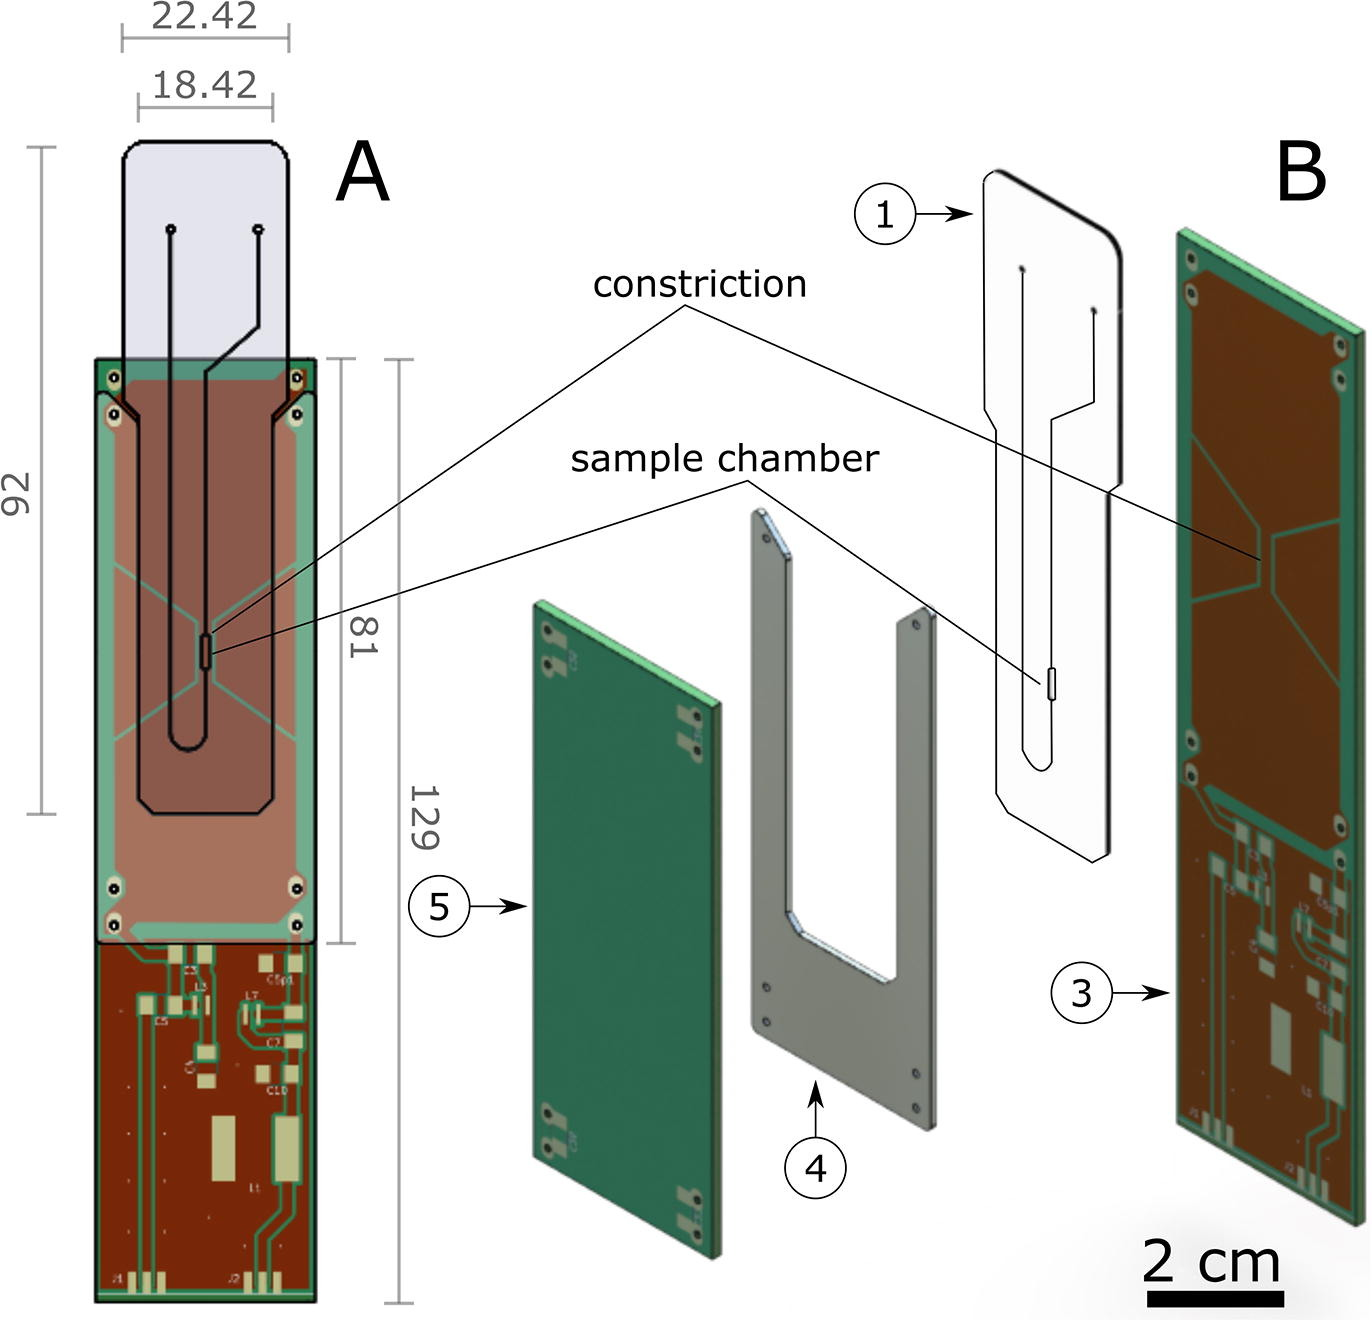
\includegraphics[width=\columnwidth]{Manvendra-Probe.jpg}
  \end{center}
  \caption{Drawings of the detector assembly and the microfluidic device (1). A: front view (dimensions in mm); B:
  exploded view. Spacer (4) ensures the alignment of the sample chamber with the constrictions on the PCB planes. In A,
  PCB plane 5 is hidden to show the orientation of 1 with respect to PCB plane 3. Thickness of each of the PCB planes
  is 1.52 mm and the copper layers on the PCBs is 35 $\mu~\text{m}$. Both the microfluidic device and the spacer are made from
  PMMA and have thickness of 0.9 mm and 1 mm respectively. Figure reproduced from\citep{RN164}}
  \label{fig:MVProbe}
\end{figure}
The main advantage of using this probe is the compatibility of the device with customisable chips allowing
a broad range of applications and enabling the marrying of practical NMR and some microfluidic capabilities which
few others allow\citep{RN165,RN166,RN167}. The limit of detection LOD for the TLP used is
1.4 nmol $\text{s}^{1/2}$ which comparitavely lower than detectors of a similar size and more similar to the LOD of
commercial cryo-probes mentioned previously. Where the probe is exceptional in terms of micro-detector is
the cLOD, this is demonstrated in \fig{fig:cLOD} which shows a wide variety of micro-NMR detectors that have been reported in the literature. \fig{fig:cLOD} has detection volume and mass LOD (nLOD) plotted logarithmically
on the $x$-axis and $y$-axis respectively, the lines of gradient 1 depict lines of constant concentration (cLOD). The general trend of decreasing nLOD with size is indicated with a line of gradient $1/2$. The area shaded orange that is defined as the 'metabolomics feasible' range is a maximum 5 mM $\sqrt{\text{s}}$
ensuring species present at 0.1 mM can be detected within less than 20 mins to a sufficient resolution. The TLP has a cLOD of
~ 1 mM $\sqrt{\text{s}}$ and can detect species at 0.02 mM in that time frame. Whilst this is suitable for some metabolomic information to be
gained, however, the subtle changes in molecules present at less than 0.02 mM are of interest but
are unreachable with this probe at this time
\begin{figure}
  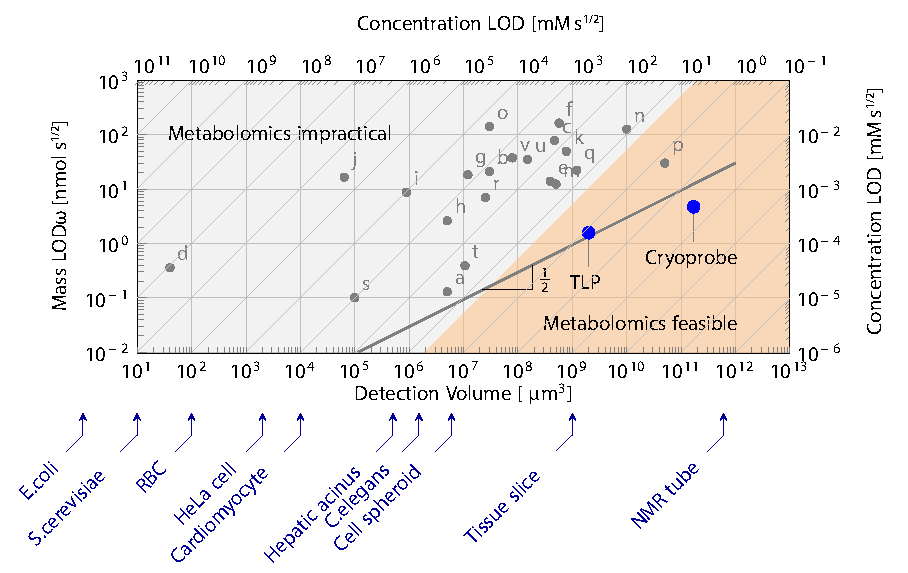
\includegraphics[width=\columnwidth]{sensitivity-ov.pdf}
  \caption{Plot comparing the limits of detection of previously design micro-NMR detectors. Letters
  a-t correspond to different authors as cited by Badilita \textit{et al.}\citep{Badilita:2011td} Letters u\citep{Meier:2014ds}
  and t\citep{RN165} represent more recent work. The probe used here is labelled at TLP and a comercial cyroprobe is shown for reference.}
  \label{fig:cLOD}
\end{figure}

For this work, the goal is not only to combine NMR detection and microfluidics, clearly that has been done before. However,
it is the combination of these two in a way that does not comprimise in either. That, in an NMR sense, means nLODs
comparible to macroprobes as well as sub 0.01 ppm line widths for true spectral resoltuion. The main
challenge, as in most NMR, is decreasing the limits of detection. Efforts towards
lowering the nLOD and cLOD are described in \ref{Chapter:Parahydrogen}
